\chapter{Neural Network Architectures}

%==============================================================================
%
%==============================================================================
\section{Feed Forward Networks}
A Feed Forward Neural Network (FFNN) is the simplest type of artificial neural network. It consists of layers of neurons where each neuron in one layer is connected to every neuron in the next layer. The information moves in one direction—forward—from the input nodes through the hidden layers (if any) to the output nodes.

FFNNs are commonly used for tasks like regression and classification. A simple implementation in Python using PyTorch is shown below.

\begin{figure}[ht]
    \centering
    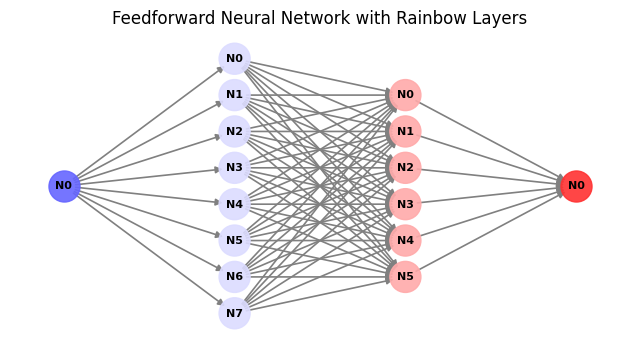
\includegraphics[width=0.7\textwidth]{images/feed_forward_network.png}
    \caption{Visualization of a simple Feedforward Neural Network (FFNN) with one hidden layer. The input, hidden, and output layers are aligned from left to right, with connections representing weight relationships.}
    \label{fig:feed_forward_network}
\end{figure}

\begin{codeonly}{Feed Forward Network}
import torch
import torch.nn as nn
import torch.optim as optim

# Define a deeper FFNN with two hidden layers
class FeedForwardNN(nn.Module):
    def __init__(self, input_size, hidden_size1, hidden_size2, output_size):
        super(FeedForwardNN, self).__init__()
        self.fc1 = nn.Linear(input_size, hidden_size1)
        self.relu1 = nn.ReLU()
        self.fc2 = nn.Linear(hidden_size1, hidden_size2)
        self.relu2 = nn.ReLU()
        self.fc3 = nn.Linear(hidden_size2, output_size)

    def forward(self, x):
        x = self.fc1(x)
        x = self.relu1(x)
        x = self.fc2(x)
        x = self.relu2(x)
        x = self.fc3(x)
        return x

# Create a model instance with 1 input, 8 neurons in the first hidden layer, 
# 6 neurons in the second hidden layer, and 1 output
input_size, hidden_size1, hidden_size2, output_size = 1, 8, 6, 1
model = FeedForwardNN(input_size, hidden_size1, hidden_size2, output_size)

# Print model architecture
print(model)
\end{codeonly}

A feedforward neural network (FFNN) consists of layers of interconnected neurons that transform input data into predictions. In this implementation, the network has an input layer with one neuron, two hidden layers with eight and six neurons, respectively, and an output layer with a single neuron. Each hidden layer applies a ReLU activation function to introduce non-linearity, enabling the model to learn complex relationships. The final output layer performs a linear transformation. 

The weights and biases of the network are learned during training through backpropagation, minimizing a chosen loss function. PyTorch's `nn.Linear` modules define fully connected layers, while the `forward` method specifies how data flows through the network. The model instance is created with predefined input, hidden, and output dimensions, and printing it reveals its architecture.

We now use such a feedforward network to approximate a non-linear curve. 

\begin{codeonly}{Learning a curve with FFNN}
import torch
import torch.nn as nn
import torch.optim as optim
import numpy as np
import matplotlib.pyplot as plt

# Set random seed & generate data: f(x) = 1 / (1 + exp(-tau * x + s))
torch.manual_seed(42); np.random.seed(42)
x = np.linspace(-2, 2, 500)
y = 1 / (1 + np.exp(-5 * x))  # tau = 5, s = 0
x_tensor = torch.tensor(x, dtype=torch.float32).unsqueeze(1)
y_tensor = torch.tensor(y, dtype=torch.float32).unsqueeze(1)

# Define a deeper FFNN
class DeepFFNN(nn.Module):
    def __init__(self):
        super().__init__()
        self.fc1, self.fc2, self.fc3 = nn.Linear(1, 8), nn.Linear(8, 6), nn.Linear(6, 1)
    def forward(self, x): return self.fc3(torch.relu(self.fc2(torch.relu(self.fc1(x)))))

model = DeepFFNN()
criterion = nn.MSELoss()
optimizer = optim.Adam(model.parameters(), lr=0.01)

# Training
loss_history = []
for epoch in range(2000):
    optimizer.zero_grad()
    y_pred = model(x_tensor)
    loss = criterion(y_pred, y_tensor)
    loss.backward()
    optimizer.step()
    loss_history.append(loss.item())
    if (epoch + 1) % 500 == 0: print(f"Epoch {epoch+1}, Loss: {loss.item():.6f}")

# Generate predictions
with torch.no_grad(): y_pred_np = model(x_tensor).numpy()

# Plot function approximation & loss curve
fig, axes = plt.subplots(1, 2, figsize=(10, 3))
axes[0].plot(x, y, label="True", linewidth=2)
axes[0].plot(x, y_pred_np, "r--", label="NN Approx.", linewidth=2)
axes[0].set(title="Function Approximation", xlabel="x", ylabel="f(x)"); axes[0].legend(); axes[0].grid()
axes[1].semilogy(loss_history, "r", label="Loss")
axes[1].set(title="Loss Curve", xlabel="Epochs", ylabel="MSE"); axes[1].legend(); axes[1].grid()
plt.savefig("deep_nn_results.png")
plt.show()
\end{codeonly}

\begin{figure}[ht]
    \centering
    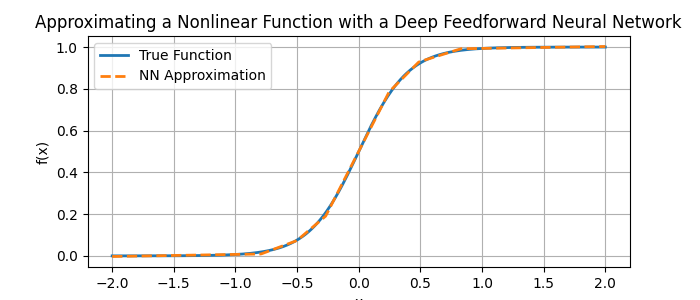
\includegraphics[width=0.48\textwidth]{images/deep_nn_function_approximation.png}
    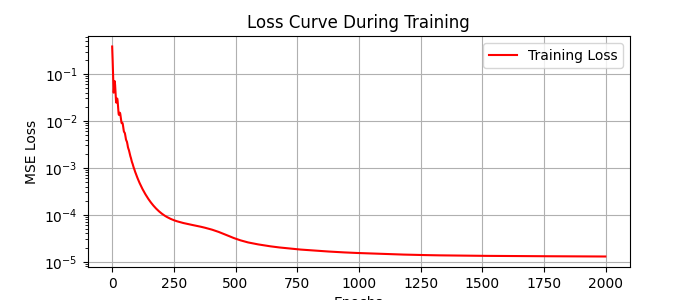
\includegraphics[width=0.48\textwidth]{images/deep_nn_loss_curve.png}
    \caption{Left: Neural network approximation of the function \( f(x) = \frac{1}{1 + e^{-\tau x + s}} \). 
    Right: Training loss curve over epochs, showing convergence of the model.}
    \label{fig:nn_function_loss}
\end{figure}

A computational graph visually represents how data flows through a neural network during a forward pass. In this example, we use the \texttt{torchviz} library to generate a graph of the feedforward neural network (FFNN). The input tensor is a randomly generated vector with the same dimensionality as the input layer. The forward pass computes the predicted output, which is then passed to \texttt{make\_dot()} along with the model’s parameters. The resulting graph shows the dependencies between layers and operations, helping to analyze the network structure and gradient flow.

\begin{codeonly}{Generating a Computational Graph}
from torchviz import make_dot

# Sample input tensor (random data)
x = torch.randn(1, input_size)  # One sample with 1 feature
y_pred = model(x)  # Forward pass

# Create the computational graph
dot = make_dot(y_pred, params=dict(model.named_parameters()))

# Render the graph
dot.render("ffnn_graph", format="png", cleanup=True)
dot
\end{codeonly}

\begin{figure}
    \centering
    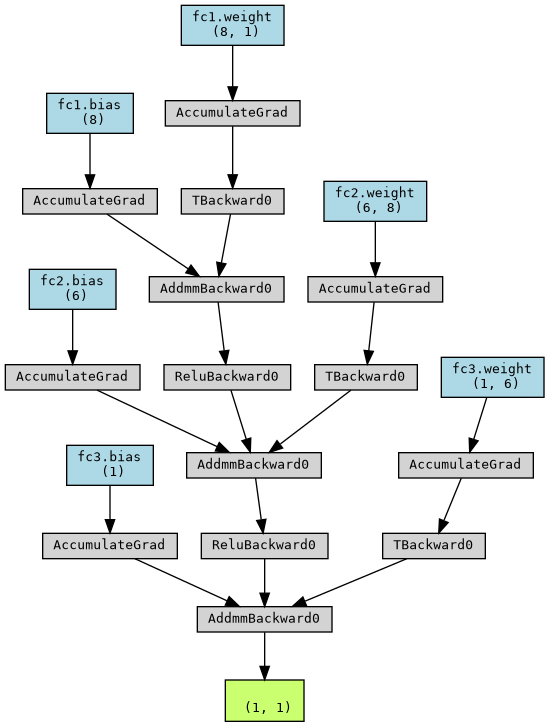
\includegraphics[width=0.6\textwidth]{images/ffnn_graph.png}
    \caption{Computational graph of the feedforward neural network.}
\end{figure}

Each box in the computational graph represents a tensor operation within the neural network. The nodes labeled \textbf{Addmm} correspond to the linear transformations performed by the \texttt{nn.Linear} layers, which compute matrix multiplications followed by bias addition. The \textbf{Relu} nodes apply the ReLU activation function, introducing non-linearity into the network. 

The parameters of the network, such as weights and biases, are indicated separately and contribute to the forward computation. This visualization helps trace how data propagates through the layers and identifies where gradients will be computed during backpropagation.

In the computational graph, \textbf{Accumulated Grad} represents the storage of gradients during backpropagation. When computing the gradient of the loss with respect to model parameters, PyTorch accumulates these gradients in the \texttt{.grad} attribute of tensors, allowing optimization steps to adjust weights accordingly.

\textbf{AddmmBackward} corresponds to the backward operation of the \textbf{Addmm} function, which performs matrix multiplication followed by bias addition in the forward pass. During backpropagation, \textbf{AddmmBackward} computes the gradients of the output with respect to both the input features and the weight matrices of the fully connected layers. These gradients are then accumulated and used for parameter updates during training.

%==============================================================================
%
%==============================================================================
\section{Graph Neural Networks}

Graph Neural Networks (GNNs) are designed to work with graph-structured data. Unlike FFNNs, GNNs can capture relationships between different entities in a graph, making them useful in applications such as social network analysis, molecular property prediction, and recommendation systems.

\begin{figure}[h!]
    \centering
    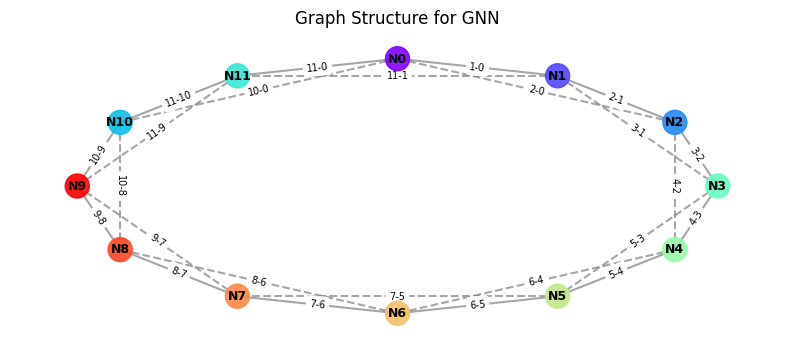
\includegraphics[width=0.8\textwidth]{images/gnn_graph.png}
    \caption{Graph visualization for the GNN model with periodic connectivity and elliptical node positions. The nodes are positioned on an ellipse, and the edges are displayed with two types: straight edges (direct neighbors) and periodic edges (non-direct neighbors).}
    \label{fig:gnn_graph}
\end{figure}

A simple implementation using PyTorch Geometric is shown below. I could get this easily running on linux, on my windows wls, on colab and other frameworks, but on Windows it died regularly without error message. Seems to be a memory management problem. 

\begin{recommendationbox}
Training with pytorch or pytorch lightning packages or any other current AI/ML software is characterized by frequent software updates. You will need to move along with the community in a timescale of month, packages get depreciated soon. 
\end{recommendationbox}

\begin{codeonly}{Graph Neural Network}
import torch
import torch.nn as nn
import torch.nn.functional as F
from torch_geometric.nn import GCNConv
from torch_geometric.data import Data

# Define a GNN with 2 hidden layers
class GNNModel(nn.Module):
    def __init__(self, num_features, hidden_channels, num_feats_y):
        super().__init__()
        self.conv1, self.conv2 = GCNConv(num_features, hidden_channels[0]), GCNConv(hidden_channels[0], hidden_channels[1])
        self.fc1, self.fc2 = nn.Linear(hidden_channels[1], hidden_channels[0]), nn.Linear(hidden_channels[0], num_feats_y)

    def forward(self, x, edge_index):
        x = F.leaky_relu(self.conv1(x, edge_index))
        x = F.leaky_relu(self.conv2(x, edge_index))
        x = F.leaky_relu(self.fc1(x))
        return self.fc2(x)

# Graph Configuration
nx, xa = 25, 10
x_grid = torch.linspace(0, xa, nx)
p1, p2 = torch.sin(2 * torch.pi * x_grid / xa), torch.cos(2 * torch.pi * x_grid / xa)

# Create adjacency matrix & edge index
diff = torch.sqrt((p1.repeat(nx, 1).T - p1) ** 2 + (p2.repeat(nx, 1).T - p2) ** 2)
edge_index = (diff < 0.5).float().nonzero(as_tuple=False).t().contiguous()

# Create node features & labels
data = Data(x=torch.cat((p1.unsqueeze(1), p2.unsqueeze(1)), dim=1), y=torch.randint(0, 2, (nx, 1)).float(), edge_index=edge_index)

# Initialize & print model
model = GNNModel(num_features=2, hidden_channels=[8, 16], num_feats_y=1)
print(model)
\end{codeonly}

Here, the edge index is for each node given by its index (first row) it prescribes the connected node by index in the second row.  
\begin{codeonly}{edge\_index}
tensor([[ 0,  0,  0,  0,  1,  1,  1,  1,  2,  2,  2,  2,  3,  3,  3,  3,  4,  4,
          4,  4,  5,  5,  5,  5,  6,  6,  6,  6,  7,  7,  7,  7,  8,  8,  8,  8,
          9,  9,  9,  9, 10, 10, 10, 10, 11, 11, 11, 11],
        [ 1,  2, 10, 11,  0,  2,  3, 11,  0,  1,  3,  4,  1,  2,  4,  5,  2,  3,
          5,  6,  3,  4,  6,  7,  4,  5,  7,  8,  5,  6,  8,  9,  6,  7,  9, 10,
          7,  8, 10, 11,  0,  8,  9, 11,  0,  1,  9, 10]])
\end{codeonly}

\begin{figure}[h!]
    \centering
    \begin{minipage}{0.45\textwidth}
        \centering
        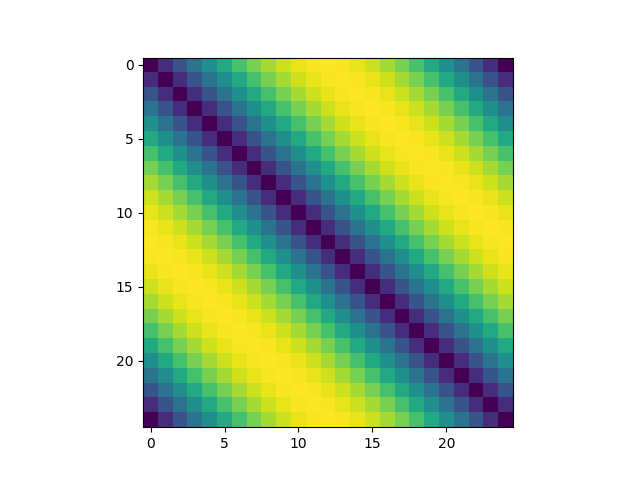
\includegraphics[width=\textwidth]{images/diff_matrix.png}
        \caption{The difference matrix showing the distances between nodes in the graph. This matrix is used to determine the adjacency matrix, where the distance between nodes is calculated based on their positions in the space.}
        \label{fig:diff_matrix}
    \end{minipage} \hfill
    \begin{minipage}{0.45\textwidth}
        \centering
        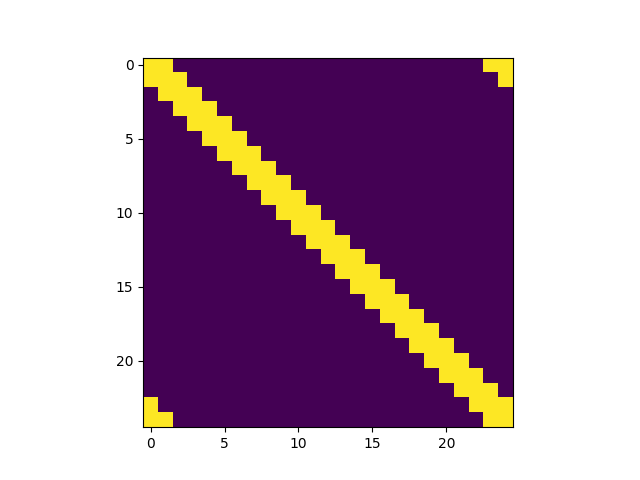
\includegraphics[width=\textwidth]{images/diff_matrix_smaller_const.png}
        \caption{A binary adjacency matrix where edges are drawn between nodes whose distance is less than 0.5. This matrix is used to determine which nodes are directly connected in the graph.}
        \label{fig:diff_matrix_smaller}
    \end{minipage}
\end{figure}

We finally show how we can learn the {\bf advection} of functions by a the above graph neural network. 

\begin{codeonly}{Training code}
import numpy as np
import matplotlib.pyplot as plt
import torch
import torch.nn as nn
import torch.nn.functional as F
import torch_geometric.data as geom_data
import torch_geometric.nn as geom_nn

# Set random seed
torch.manual_seed(0)

# Define parameters
xa, nx, nt, v = 10, 25, 15, 0.6

# Create grid and function data
x_grid = np.linspace(0, xa, nx + 1)[:-1]
z = np.zeros([nt, nx])
for j in range(nt):
    z[j, :] = np.sin((2 * np.pi / xa) * x_grid - v * j)

# Create adjacency matrix
p1 = np.sin(2 * np.pi * x_grid / xa)
p2 = np.cos(2 * np.pi * x_grid / xa)
p1m, p2m = np.tile(p1, (nx, 1)).T, np.tile(p2, (nx, 1)).T
diff = np.sqrt((p1m - p1m.T) ** 2 + (p2m - p2m.T) ** 2)
adjm = (diff < 0.5).astype(int)
edge_index = torch.tensor(np.nonzero(adjm), dtype=torch.long)

# Split data into training and testing
X_train, Y_train = z[:-1], z[1:]
X_test, Y_test = z[:-1], z[1:]

# Create feature tensors and data loader
features_tmp2 = torch.tensor(np.arange(1, nx + 1) / nx, dtype=torch.float).unsqueeze(1)
train_list, test_list = [], []
for k in range(X_train.shape[0]):
    features_k_tmp1 = torch.tensor(X_train[k, :], dtype=torch.float).unsqueeze(1)
    features_k = torch.cat((features_k_tmp1, features_tmp2), dim=1)
    labels_k = torch.tensor(Y_train[k, :], dtype=torch.float).unsqueeze(1)
    data = geom_data.Data(x=features_k, y=labels_k, edge_index=edge_index)
    train_list.append(data)

for k in range(X_test.shape[0]):
    features_k_tmp1 = torch.tensor(X_test[k, :], dtype=torch.float).unsqueeze(1)
    features_k = torch.cat((features_k_tmp1, features_tmp2), dim=1)
    labels_k = torch.tensor(Y_test[k, :], dtype=torch.float).unsqueeze(1)
    data = geom_data.Data(x=features_k, y=labels_k, edge_index=edge_index)
    test_list.append(data)

# Create DataLoaders for training and testing
train_loader = geom_data.DataLoader(train_list, batch_size=1, shuffle=True)
test_loader = geom_data.DataLoader(test_list, batch_size=1, shuffle=False)

# Define the GNN model
class GNNModel(nn.Module):
    def __init__(self, num_features, hidden_channels, num_feats_y):
        super(GNNModel, self).__init__()
        self.conv1 = geom_nn.GCNConv(num_features, hidden_channels[0])
        self.conv2 = geom_nn.GCNConv(hidden_channels[0], hidden_channels[1])
        self.conv3 = geom_nn.GCNConv(hidden_channels[1], hidden_channels[2])
        self.conv4 = geom_nn.GCNConv(hidden_channels[2], hidden_channels[3])
        self.fc1 = nn.Linear(hidden_channels[3], hidden_channels[2])
        self.fc2 = nn.Linear(hidden_channels[2], hidden_channels[0])
        self.fc3 = nn.Linear(hidden_channels[0], num_feats_y)

    def forward(self, x, edge_index):
        x = F.leaky_relu(self.conv1(x, edge_index))
        x = F.leaky_relu(self.conv2(x, edge_index))
        x = F.leaky_relu(self.conv3(x, edge_index))
        x = F.leaky_relu(self.conv4(x, edge_index))
        x = F.leaky_relu(self.fc1(x))
        x = F.leaky_relu(self.fc2(x))
        return self.fc3(x)

# Initialize model, optimizer, and criterion
model = GNNModel(num_features=2, hidden_channels=[4 * nt, 4 * nt, 4 * nt, 4 * nt], num_feats_y=1)
optimizer = torch.optim.AdamW(model.parameters(), lr=0.0005, weight_decay=0)
criterion = nn.MSELoss()

# Training loop
epochs = 1500
train_mse, test_mse = [], []
for epoch in range(epochs):
    model.train()
    total_loss = 0.0
    train_mse_tmp = []
    for batch in train_loader:
        optimizer.zero_grad()
        output = model(batch.x, batch.edge_index)
        loss = criterion(output, batch.y)
        train_mse_tmp.append(loss.item())
        loss.backward()
        optimizer.step()
    train_mse.append(np.mean(train_mse_tmp))

    model.eval()
    test_mse_tmp = []
    for batch in test_loader:
        y_pred = model(batch.x, batch.edge_index)
        test_loss = criterion(y_pred, batch.y)
        test_mse_tmp.append(test_loss.item())
    test_mse.append(np.mean(test_mse_tmp))

    if epoch % 100 == 0:
        print(f'Epoch {epoch + 1}, Train Loss: {train_mse[epoch]}, Test Loss: {test_mse[epoch]}')

# Plot training and test MSE
plt.plot(np.arange(epochs), train_mse, '*', label='Train Loss')
plt.plot(np.arange(epochs), test_mse, '*', label='Test Loss')
plt.legend()
plt.title("Training and Test Loss")
plt.savefig("gnn_loss_curve.png")
plt.show()
\end{codeonly}

Which comes with the loss curve

\begin{figure}[h!]
    \centering
    \begin{minipage}{0.8\textwidth}
        \centering
        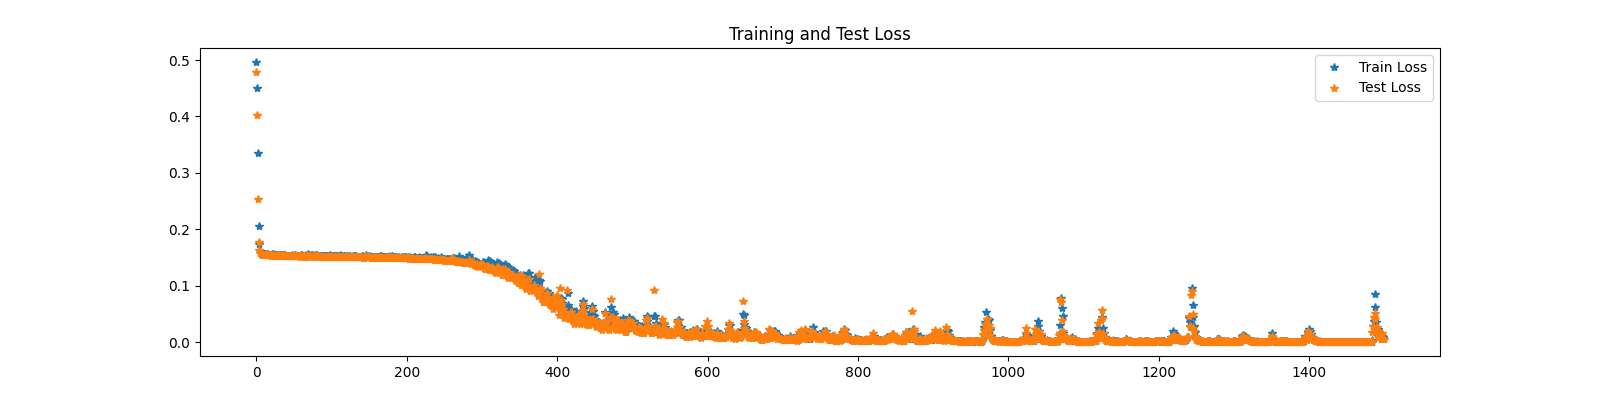
\includegraphics[width=\textwidth]{images/gnn_loss_curve.png}
        \caption{Training and Test Loss curves during the training process. The plot shows the Mean Squared Error (MSE) for both training and test sets across epochs.}
        \label{fig:gnn_test_2}
    \end{minipage}
\end{figure}

Testing the translation we display two randomly chosen cases. 

\begin{figure}[h!]
    \centering
    \begin{minipage}{0.45\textwidth}
        \centering
        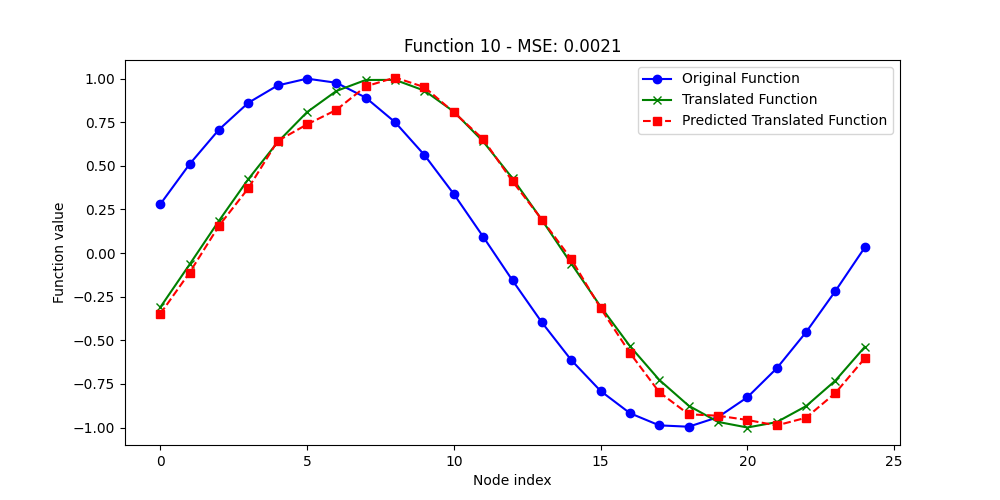
\includegraphics[width=\textwidth]{images/gnn_test_tds_1.png}
        \caption{Comparison for Test Case 1: Original, Translated, and Predicted Translated Functions. The plot shows the original function, the translated function, and the model's prediction with MSE value.}
        \label{fig:gnn_loss_curve}
    \end{minipage} \hfill
    \begin{minipage}{0.45\textwidth}
        \centering
        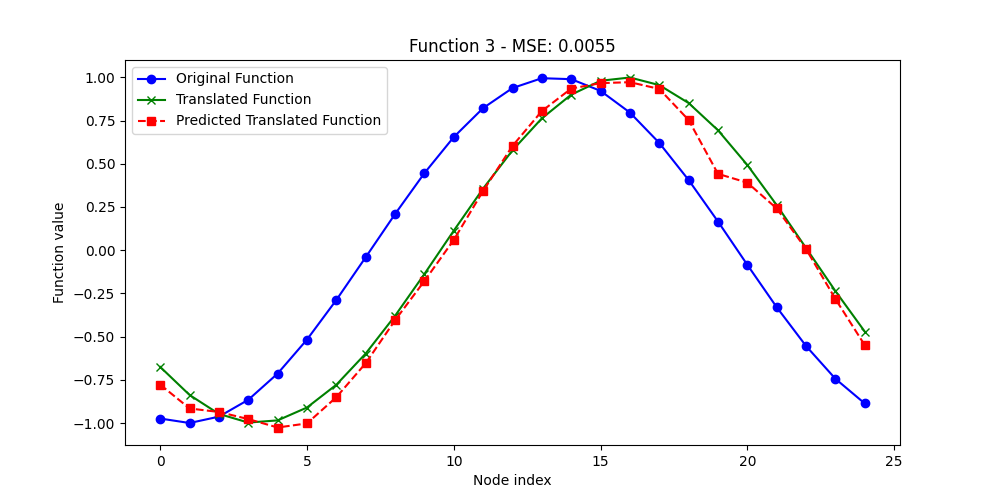
\includegraphics[width=\textwidth]{images/gnn_test_tds_2.png}
        \caption{Comparison for Test Case 2: Original, Translated, and Predicted Translated Functions. This plot compares the same as Test Case 1 but for another random test case.}
        \label{fig:gnn_test_1}
    \end{minipage}
\end{figure}



%==============================================================================
%
%==============================================================================
\section{Applying Convolutional Neural Networks for Function Classification}

Convolutional Neural Networks (CNNs) are powerful architectures typically used for image processing but can also be applied to one-dimensional data such as time series or function classification. In this section, we demonstrate how to construct a simple CNN to classify different mathematical functions (e.g., sine, cosine, Gaussian, and polynomial functions). 

{\bf Generating Synthetic Data.} To train a CNN, we first need a dataset. We generate synthetic data using functions such as sine or cosine, polynomials and Gaussians with varying parameters such as frequency, phase shifts, and noise levels. The dataset consists of labeled samples representing different mathematical function types. 

\begin{codeonly}{CNN Data generation}
import torch
import torch.nn as nn
import torch.optim as optim
import numpy as np
import matplotlib.pyplot as plt

def generate_function_data(num_samples=5000, num_points=50, err=0.02):
    X = []
    y = []
    functions = ['sine-cosine', 'gaussian', 'polynomial']
    
    for _ in range(num_samples):
        x = np.linspace(-1, 1, num_points)
        func_type = np.random.choice(functions)

        # Initialize a default y_values to prevent UnboundLocalError
        y_values = np.zeros(num_points)
        label = -1

        if func_type == 'sine-cosine':
            freq = np.random.uniform(1, 5)  
            phase = np.random.uniform(0, 2 * np.pi)
            amp = np.random.uniform(0.5, 2)
            y_values = amp * np.sin(freq * np.pi * x + phase) + err * np.random.randn(num_points)
            label = 0

        elif func_type == 'gaussian':
            mu = np.random.uniform(-0.5, 0.5)  
            sigma = np.random.uniform(0.2, 0.5)  
            amp = np.random.uniform(0.5, 2)
            y_values = amp * np.exp(-((x - mu) ** 2) / (2 * sigma ** 2)) + err * np.random.randn(num_points)
            label = 2

        elif func_type == 'polynomial':
            a = np.random.uniform(-2, 2)
            b = np.random.uniform(-2, 2)
            c = np.random.uniform(-3, 3)
            d = np.random.uniform(-0.5, 0.5)
            y_values = a * x**3 + b * x**2 + c * x + d + err * np.random.randn(num_points)
            label = 3

        X.append(y_values)
        y.append(label)

    X = np.array(X).reshape(-1, 1, num_points)  # Add channel dimension
    y = np.array(y)
    
    return torch.tensor(X, dtype=torch.float32), torch.tensor(y, dtype=torch.long)

# Generate a large training and test dataset with adjustable noise
X_train, y_train = generate_function_data(num_samples=10000, err=0.05)  # Low noise in training
X_test, y_test = generate_function_data(num_samples=2000, err=0.2)  # Higher noise in test set

print(f"Train Data Shape: {X_train.shape}, Train Labels Shape: {y_train.shape}")
print(f"Test Data Shape: {X_test.shape}, Test Labels Shape: {y_test.shape}")

plt.figure(figsize=(12, 3))
for i, idx in enumerate(torch.randperm(len(X_train))[:6]):
    plt.subplot(1, 6, i + 1)
    plt.plot(X_train[idx][0].cpu().numpy())
    plt.title([y_train[idx].item()])
    plt.xticks([]), plt.yticks([])

plt.tight_layout()
plt.savefig("cnn_data_samples.png", dpi=300)
plt.show()
\end{codeonly}
%\includeexternalcode{CNN Training Data}{chapter05/cnn_data_generation.py}

Each function is sampled over a fixed range, and the noise level can be controlled via a parameter. The generated dataset is split into training and test sets.

\begin{figure}[h]
    \centering
    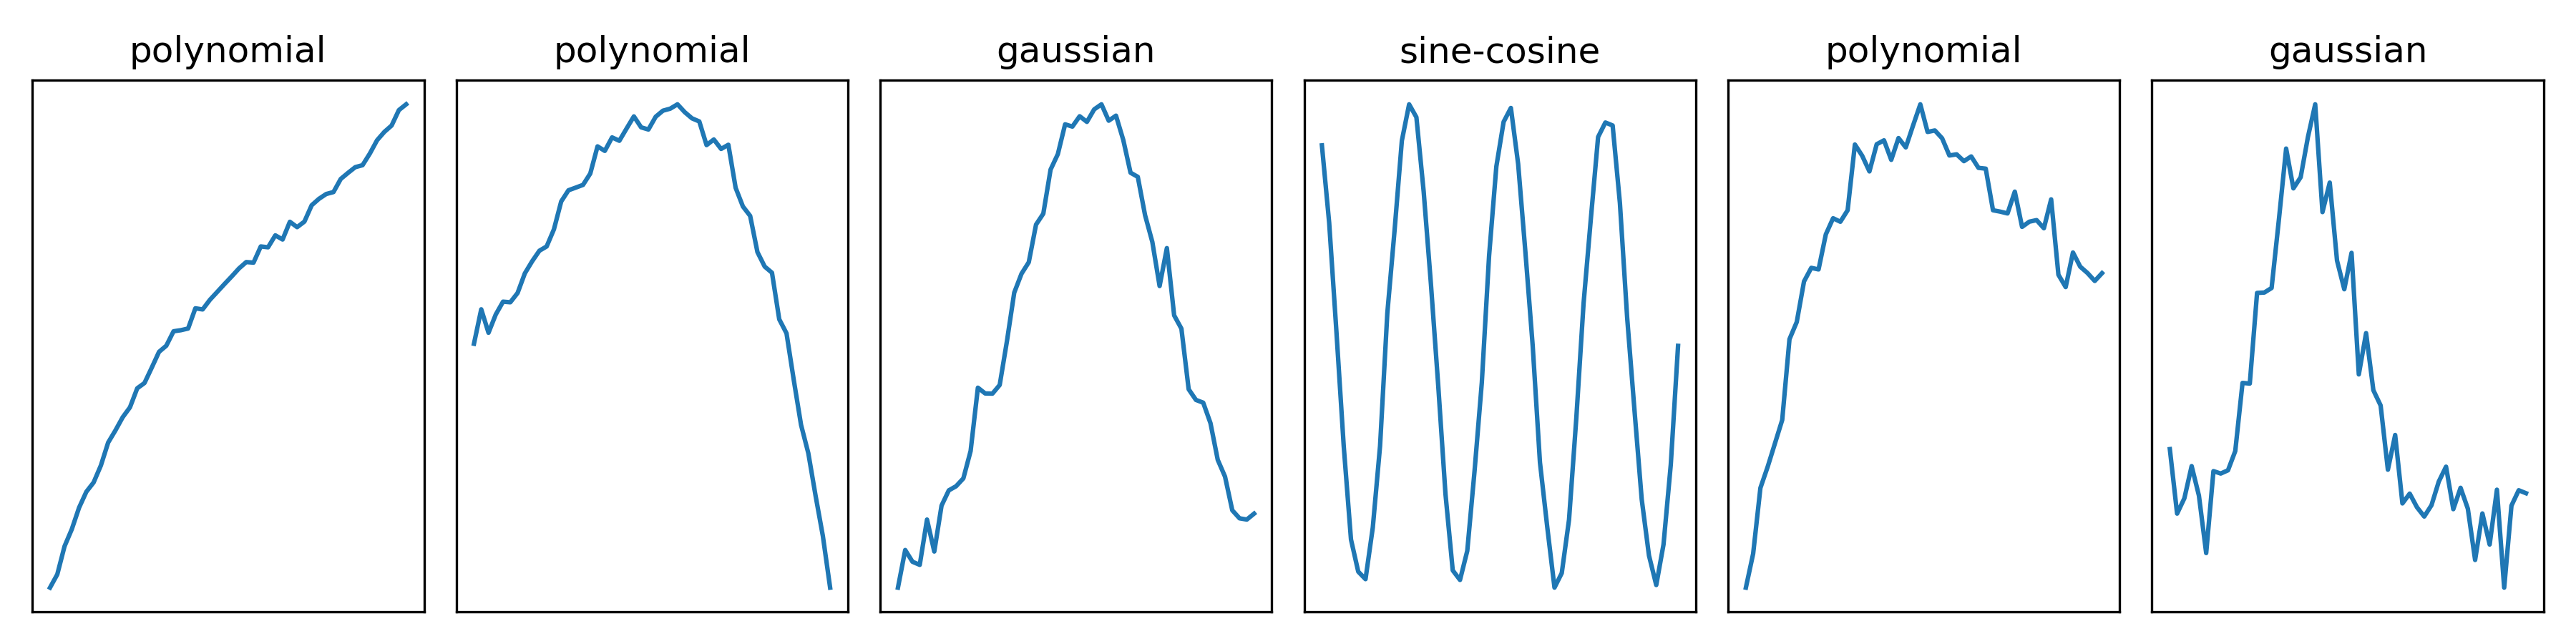
\includegraphics[width=0.8\textwidth]{images/cnn_data_samples_selected.png}
    \caption{Example of generated function data samples}
    \label{fig:data_samples}
\end{figure}

{\bf Defining the Convolutional Neural Network.} The next step is defining the CNN. Our model consists of two convolutional layers, followed by a fully connected network that maps extracted features to class labels.

\begin{codeonly}{CNN Definition}
import torch
import torch.nn as nn
import torch.optim as optim

class FunctionClassifierCNN(nn.Module):
    def __init__(self):
        super(FunctionClassifierCNN, self).__init__()
        self.conv1 = nn.Conv1d(in_channels=1, out_channels=16, kernel_size=5, stride=1, padding=2)
        self.conv2 = nn.Conv1d(in_channels=16, out_channels=32, kernel_size=5, stride=1, padding=2)
        self.fc1 = nn.Linear(32 * 50, 128)
        self.fc2 = nn.Linear(128, 4)  # 4 classes

    def forward(self, x):
        x = torch.relu(self.conv1(x))
        x = torch.relu(self.conv2(x))
        x = x.view(x.shape[0], -1)  # Flatten
        x = torch.relu(self.fc1(x))
        x = self.fc2(x)
        return x

# Initialize model
model = FunctionClassifierCNN()
print(model)
\end{codeonly}
%\includeexternalcode{CNN Definition}{chapter05/cnn_definition.py}

The convolutional layers apply feature extraction by detecting local patterns in the input functions. The final classification is performed by a fully connected layer.

{\bf Training the CNN.} The training process involves feeding the generated dataset into the CNN, computing loss using cross-entropy, and updating weights via backpropagation.

\begin{codeonly}{CNN Training}
# Training setup
device = torch.device("cuda" if torch.cuda.is_available() else "cpu")
model.to(device)

criterion = nn.CrossEntropyLoss()
optimizer = optim.Adam(model.parameters(), lr=0.001)

num_epochs = 20
batch_size = 32

# Convert dataset into DataLoader
train_loader = torch.utils.data.DataLoader(list(zip(X_train, y_train)), batch_size=batch_size, shuffle=True)

loss_history = []  # Store loss values

for epoch in range(num_epochs):
    total_loss = 0
    for batch_X, batch_y in train_loader:
        batch_X, batch_y = batch_X.to(device), batch_y.to(device)
        optimizer.zero_grad()
        loss = criterion(model(batch_X), batch_y)
        loss.backward()
        optimizer.step()
        total_loss += loss.item()
    
    loss_history.append(total_loss / len(train_loader))  # Save epoch loss
    print(f"Epoch {epoch+1}/{num_epochs}, Loss: {loss_history[-1]:.4f}")

# Plot training loss
fig=plt.figure(figsize=(10,5))
plt.plot(loss_history)
plt.xlabel("Epoch")
plt.ylabel("Loss")
plt.title("Training Loss")
plt.savefig("cnn_training_loss.png", dpi=300)
plt.show()
\end{codeonly}
%\includeexternalcode{CNN Training Loop}{chapter05/cnn_training.py}

During training, we monitor the loss function to ensure the model is learning effectively.

\begin{figure}[h]
    \centering
    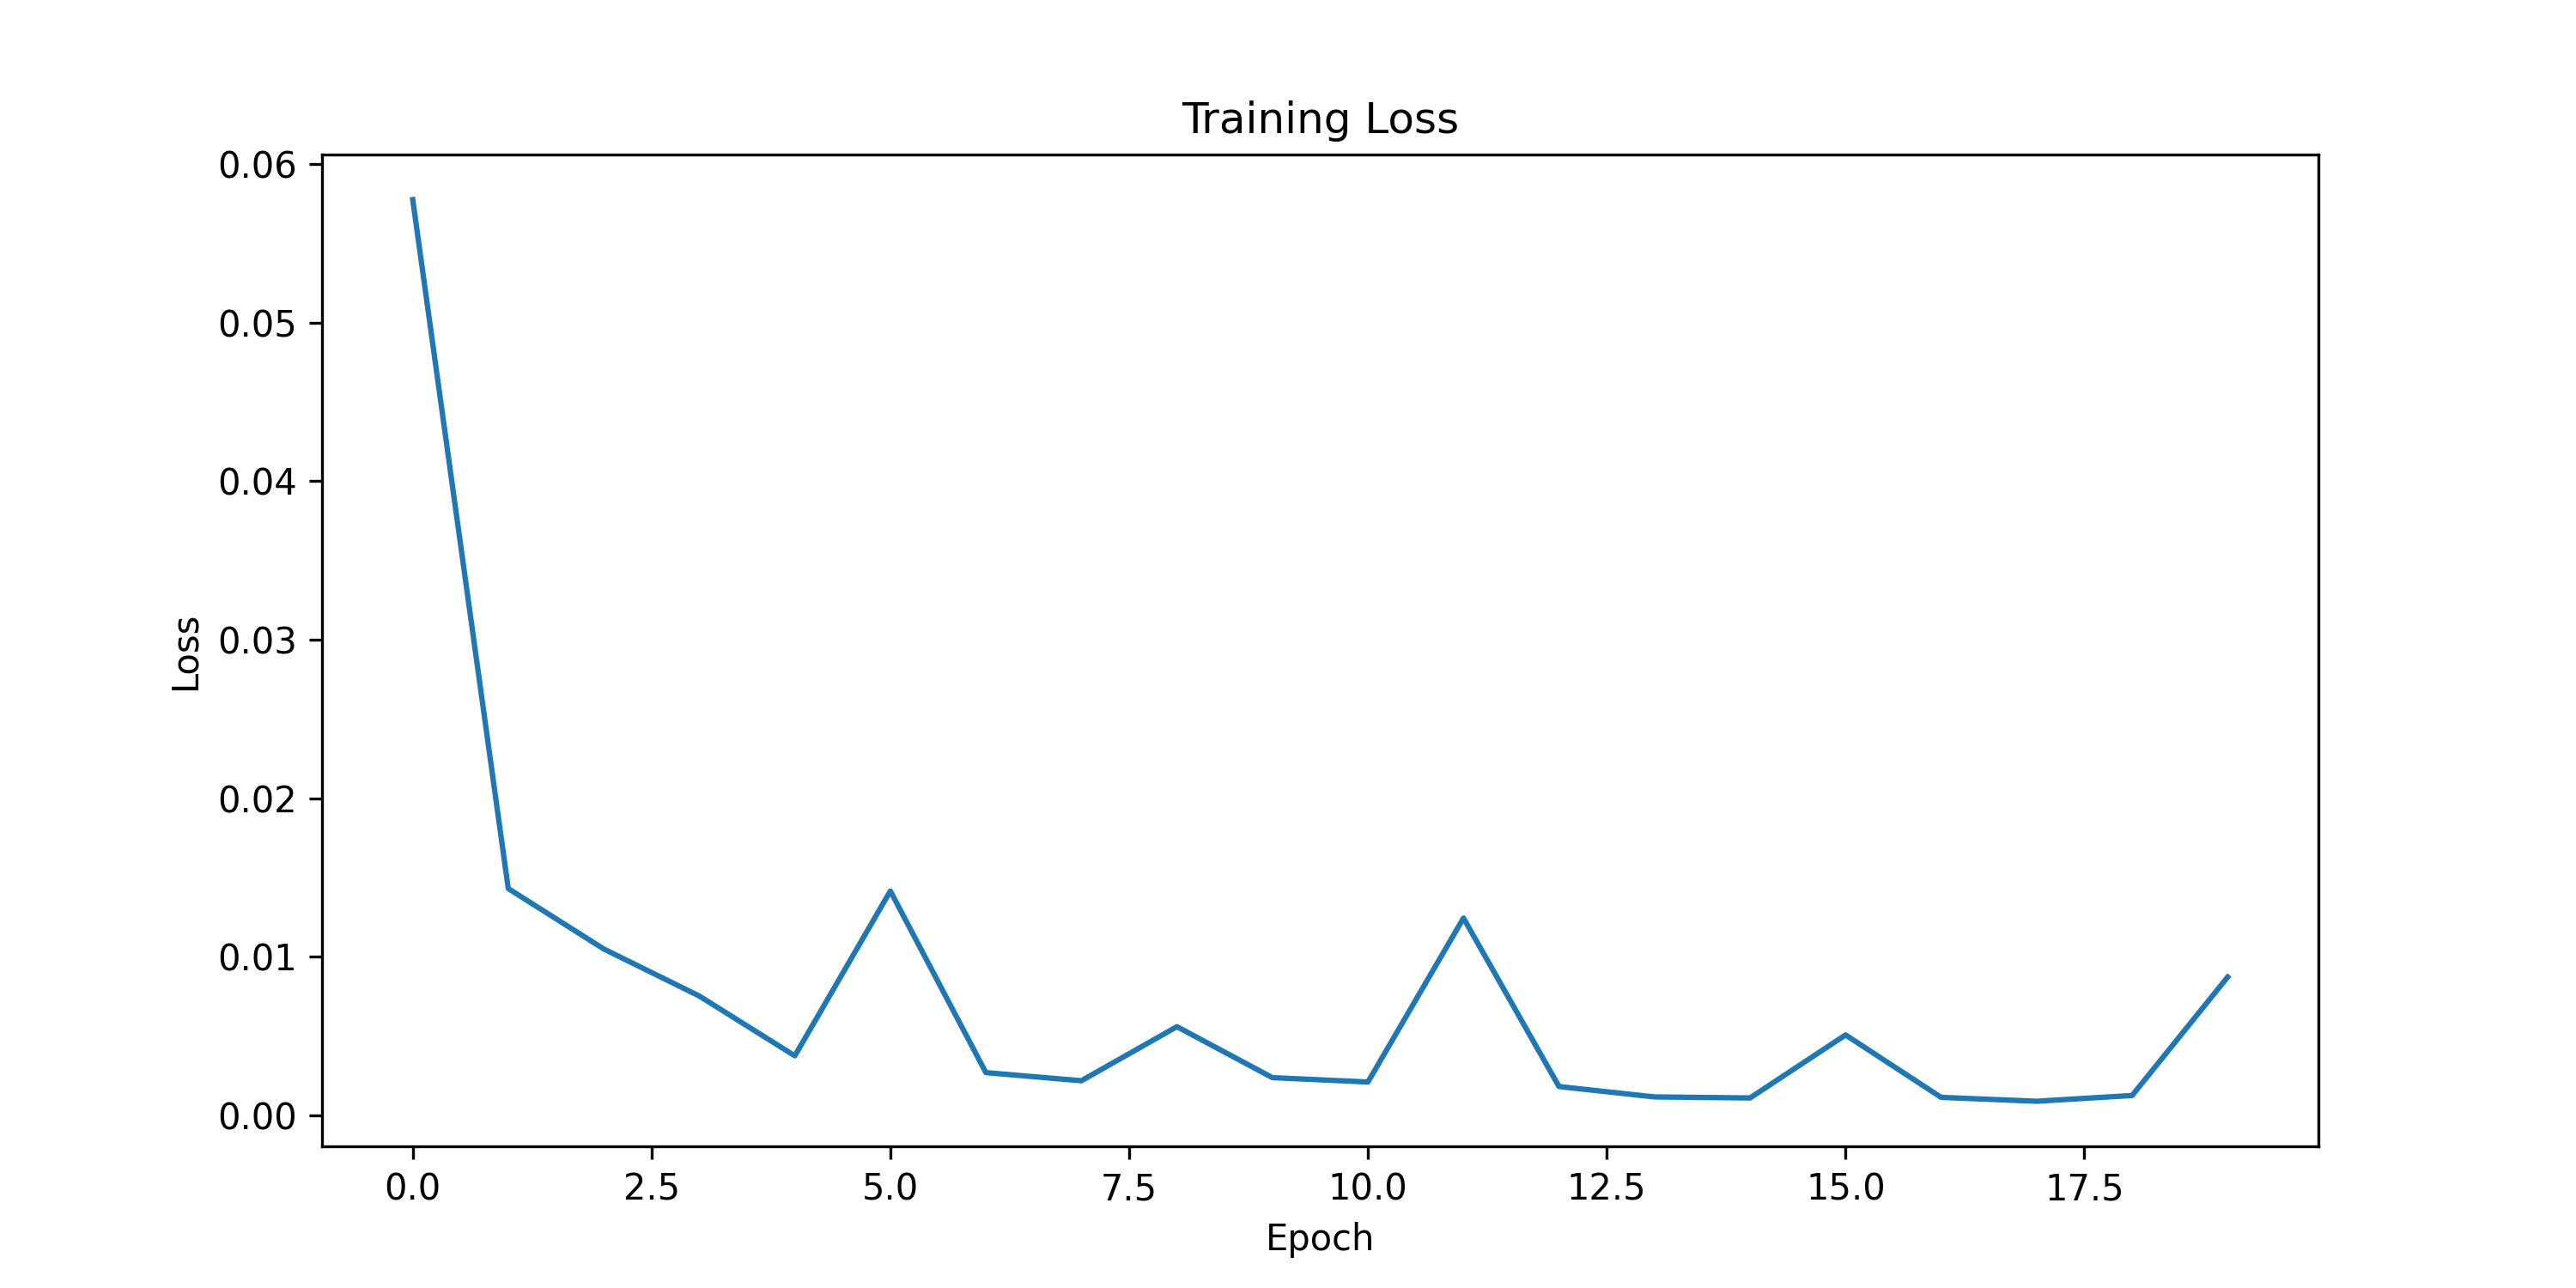
\includegraphics[width=0.8\textwidth]{images/cnn_training_loss.png}
    \caption{Training loss over epochs}
    \label{fig:training_loss}
\end{figure}

{\bf Evaluating the Model.} Once trained, the CNN is evaluated on the test dataset. Accuracy is computed to assess performance.

\begin{codeonly}{CNN Evaluation}
# Evaluation
model.eval()
test_loader = torch.utils.data.DataLoader(list(zip(X_test, y_test)), batch_size=batch_size, shuffle=False)

correct = 0
total = 0

with torch.no_grad():
    for batch_X, batch_y in test_loader:
        batch_X, batch_y = batch_X.to(device), batch_y.to(device)

        outputs = model(batch_X)
        _, predicted = torch.max(outputs, 1)

        total += batch_y.size(0)
        correct += (predicted == batch_y).sum().item()

accuracy = 100 * correct / total
print(f"Test Accuracy: {accuracy:.2f}%")
\end{codeonly}
%\includeexternalcode{Evaluation of CNN}{chapter05/cnn_evaluation.py}

A high accuracy indicates the model successfully differentiates between different function types.

{\bf Visualizing Predictions.} Finally, we visualize how well the model classifies unseen functions by plotting predicted and actual labels.

\begin{codeonly}{CNN Visualization}
import random
import matplotlib.pyplot as plt

# Generate a few test samples
num_examples = 12  # Show 12 examples
X_new, y_new = generate_function_data(num_samples=num_examples)
X_new = X_new.to(device)

# Get model predictions
model.eval()
with torch.no_grad():
    predictions = model(X_new)
    _, predicted_labels = torch.max(predictions, 1)

# Function names for visualization
func_names = ['Sine', 'Cosine', 'Gaussian', 'Polynomial']

# Plot the results
rows = num_examples // 4  # Show 4 per row
plt.figure(figsize=(12, 3 * rows))

for i in range(num_examples):
    correct = predicted_labels[i] == y_new[i]  # Check if prediction is correct
    color = 'blue' if correct else 'red'  # Blue for correct, red for incorrect

    plt.subplot(rows, 4, i + 1)
    plt.plot(np.linspace(-1, 1, 50), X_new[i].cpu().numpy().squeeze(), color=color, label=f"Pred: {func_names[predicted_labels[i]]}")
    plt.legend()
    plt.title(f"True: {func_names[y_new[i]]}", color=color)  # Color title for extra clarity
    plt.xticks([])
    plt.yticks([])

plt.tight_layout()
plt.savefig("cnn_test_predictions.png", dpi=300)
plt.show()
\end{codeonly}
%\includeexternalcode{CNN Result Visualization}{chapter05/cnn_visualization.py}

By analyzing the correctly and incorrectly classified samples, we can gain insights into model performance and potential improvements.

\begin{figure}[ht]
    \centering
    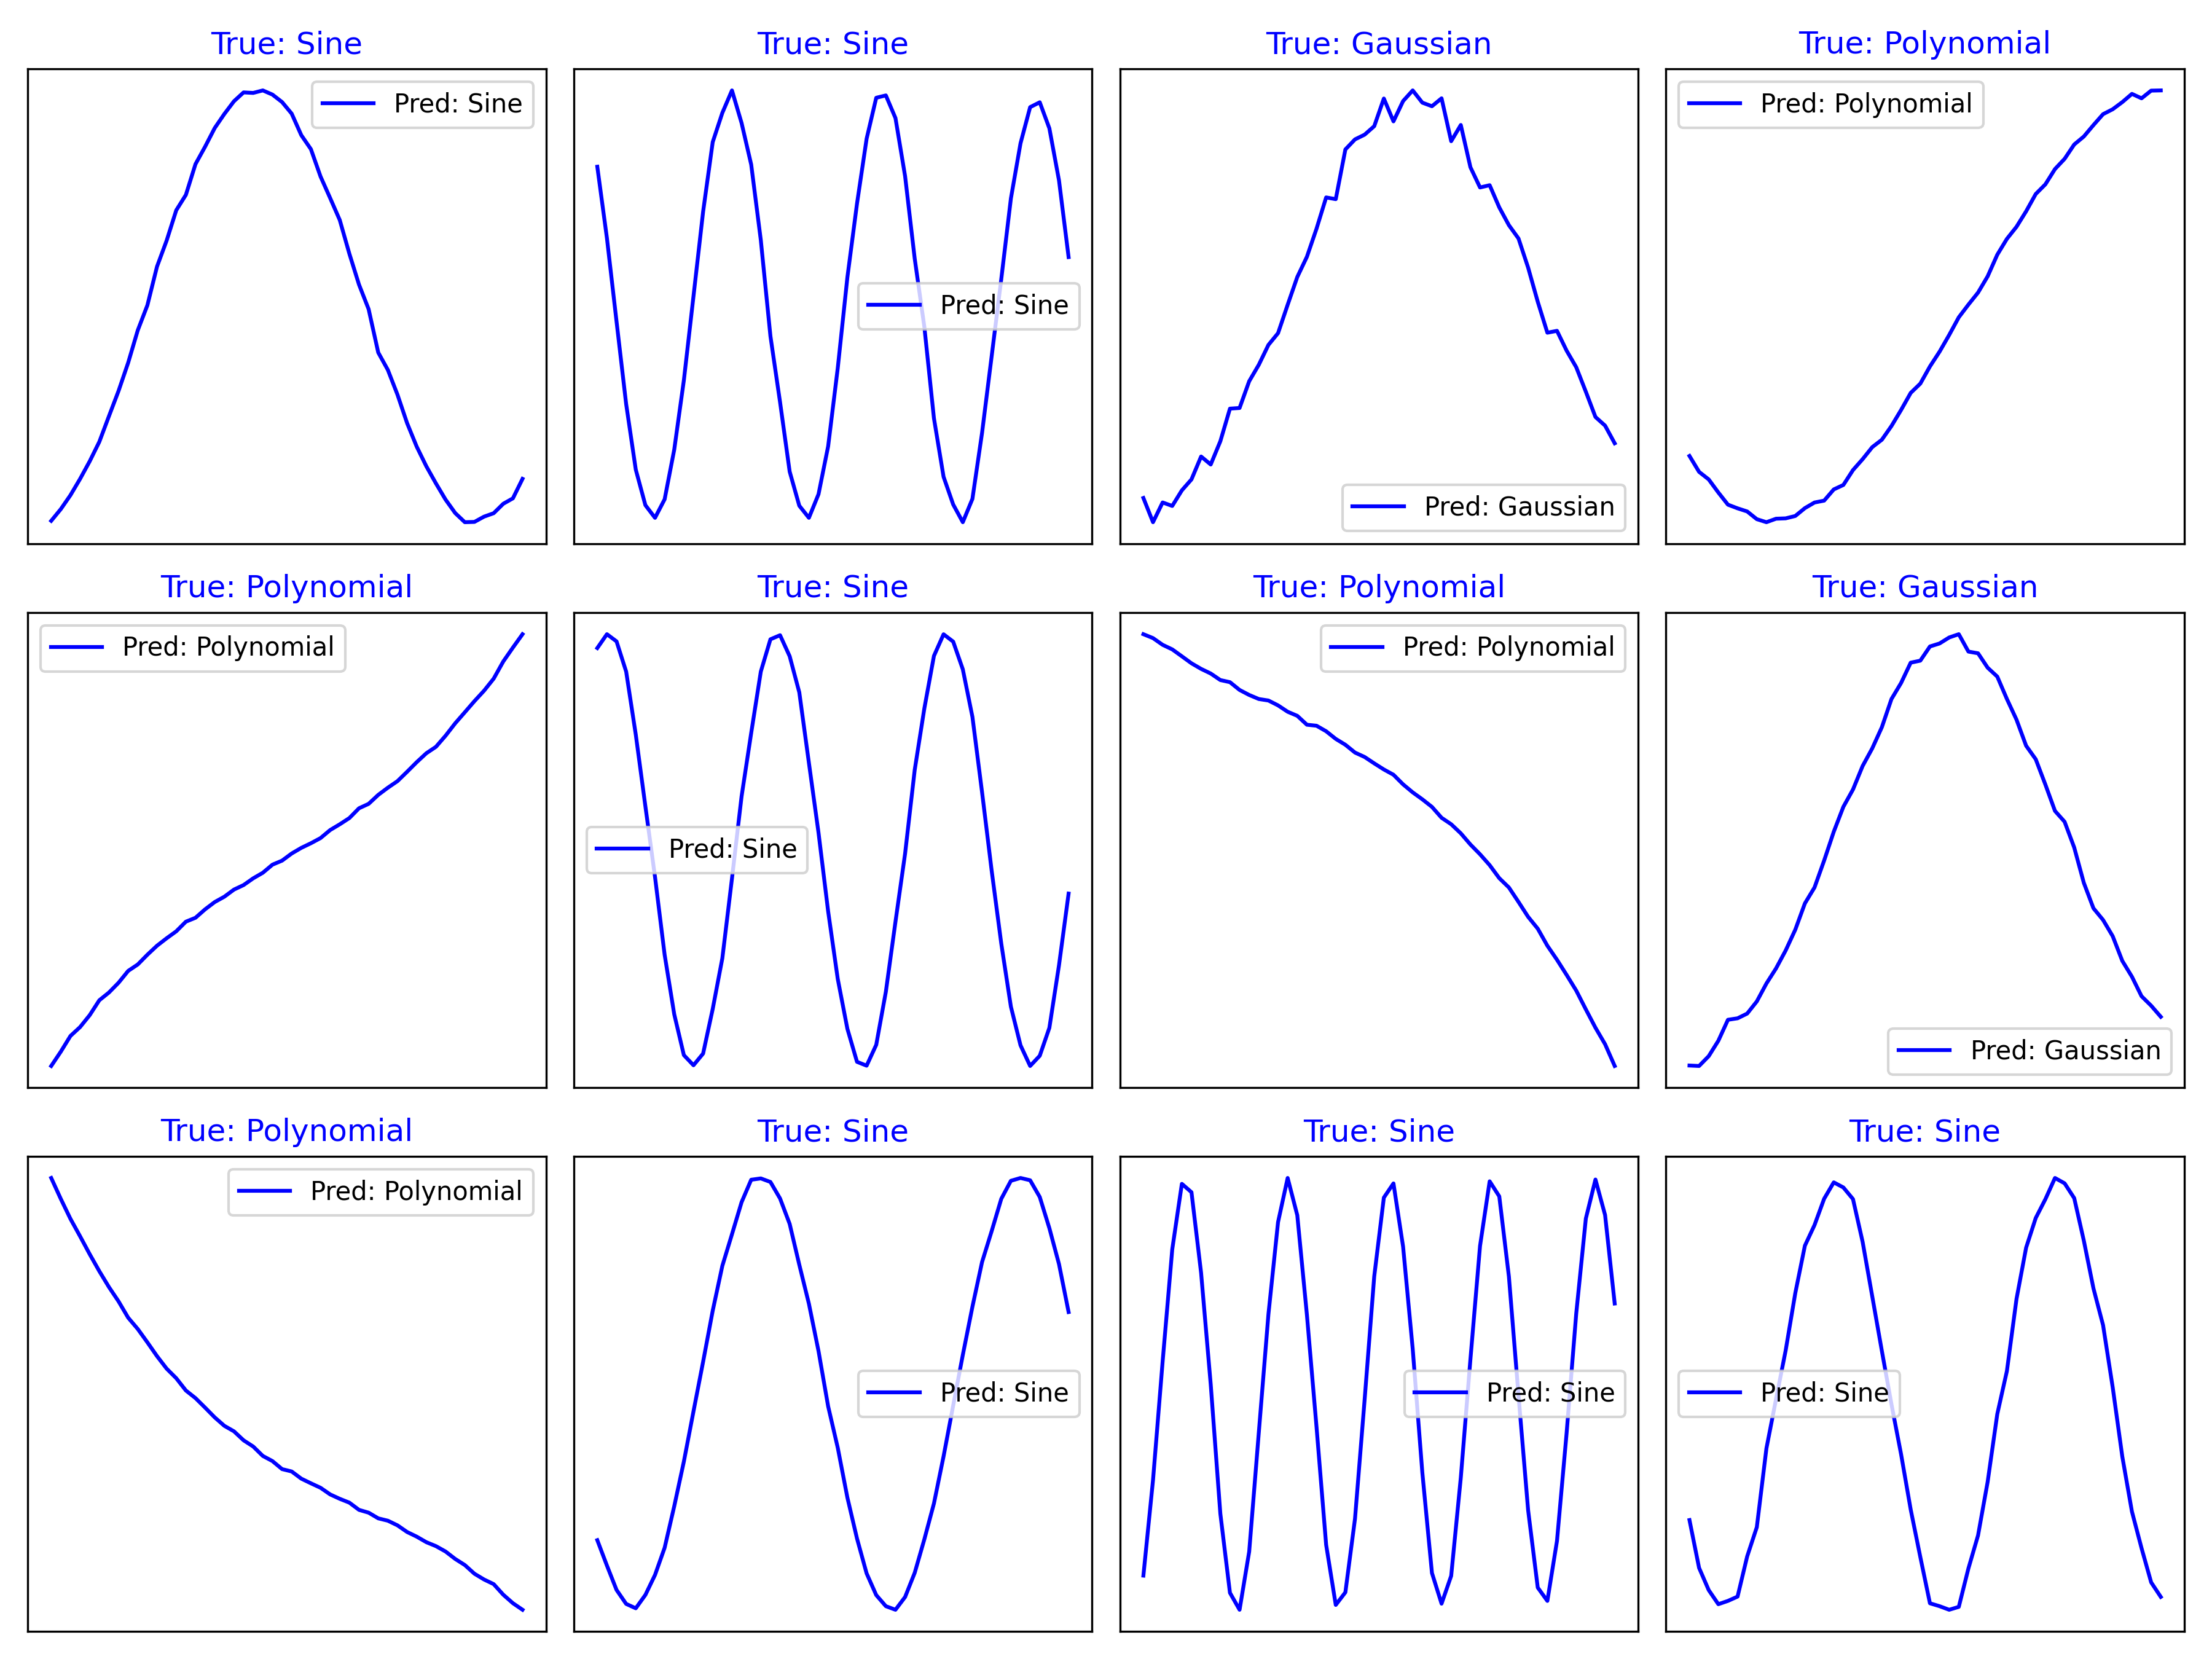
\includegraphics[width=0.8\textwidth]{images/cnn_test_predictions_select.png}
    \caption{Correct (blue) and incorrect (red) predictions}
    \label{fig:test_predictions}
\end{figure}

We have shown an application of CNNs for function classification, covering data generation, model design, training, evaluation, and visualization. This approach can be extended to classify other types of structured signals.

%==============================================================================
%
%==============================================================================
\section{LSTM-Based Anomaly Detection in Sensor Data}

Recurrent Neural Networks (RNNs), specifically Long Short-Term Memory (LSTM) networks, are powerful for handling sequential data. Unlike traditional feedforward neural networks, LSTMs are designed to capture temporal dependencies by maintaining an internal memory that allows them to remember relevant past information over long sequences. This makes them particularly suitable for anomaly detection in time series data, where deviations from learned patterns indicate potential anomalies.

An LSTM consists of a series of memory cells, each containing:
\begin{itemize}
    \item An \textbf{input gate} that determines how much new information is added to the cell state.
    \item A \textbf{forget gate} that decides what past information should be discarded.
    \item An \textbf{output gate} that controls how much information from the memory cell is used as output.
\end{itemize}
By adjusting these gates, the LSTM can selectively retain or forget information, making it highly effective at modeling sequences with long-term dependencies.

\begin{figure}[ht]
    \centering
    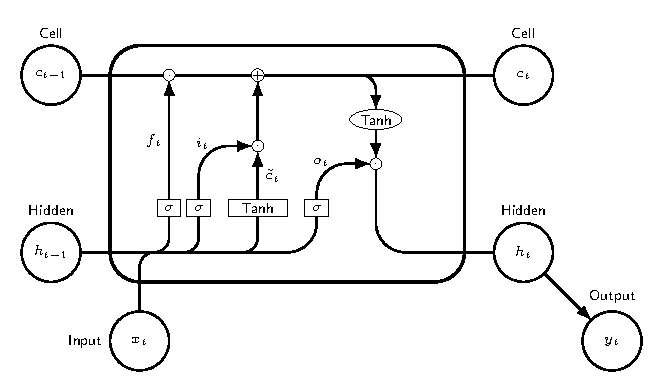
\includegraphics[width=0.6\textwidth]{chapters/lstm_graph.pdf}
    \caption{A sketch of the functionality of an LSTM cell, as described by the equations (\ref{lstm1})-(\ref{lstm7}). }
    \label{fig:lstm_graph}
\end{figure}

{\bf Mathematical Formulation of LSTM.} To be more precise, an LSTM unit consists of a cell state \( c_t \) and three gates: the input gate \( i_t \), forget gate \( f_t \), and output gate \( o_t \). The key equations governing an LSTM cell at time step \( t \) are:
\begin{eqnarray}
    f_t &= \sigma(W_f x_t + U_f h_{t-1} + b_f) \label{lstm1} \\
    i_t &= \sigma(W_i x_t + U_i h_{t-1} + b_i) \\
    o_t &= \sigma(W_o x_t + U_o h_{t-1} + b_o) \\
    \tilde{c}_t &= \tanh(W_c x_t + U_c h_{t-1} + b_c) \\
    c_t &= f_t \odot c_{t-1} + i_t \odot \tilde{c}_t \\
    h_t &= o_t \odot \tanh(c_t) \\
    y_t &= W_y h_t + b_y \label{lstm7}
\end{eqnarray}
following \href{https://arxiv.org/pdf/1506.04214}{Convolutional LSTM Network: A Machine Learning Approach for Precipitation Nowcasting}. 

Here, \( x_t \in \mathbb{R}^{m} \) represents the input at time step \( t \), while \( h_t \in \mathbb{R}^{n} \) is the hidden state, which encodes information from previous time steps. The memory cell \( c_t \in \mathbb{R}^{n} \) maintains long-term dependencies, with its update governed by three gates: the forget gate \( f_t \), which decides how much past information to retain, the input gate \( i_t \), which determines how much new information to store, and the output gate \( o_t \), which controls what is passed to the hidden state. The candidate cell state \( \tilde{c}_t \) contributes to updating \( c_t \), using weight matrices \( W_c \) and \( U_c \), and bias \( b_c \).

The weight matrices \( W_f, W_i, W_o, W_c \in \mathbb{R}^{n \times m} \) process input connections, while \( U_f, U_i, U_o, U_c \in \mathbb{R}^{n \times n} \) manage recurrent hidden state updates. Bias terms \( b_f, b_i, b_o, b_c \in \mathbb{R}^{n} \) adjust the activation functions. The element-wise sigmoid function \( \sigma \) regulates gate activations, and the hyperbolic tangent function \( \tanh \) is used for both candidate state computation and final output transformation. Element-wise multiplication is denoted by \( \odot \).

{\bf Output Computation.} The final output \( y_t \) is computed as a linear transformation \( W_y h_t + b_y \), where \( W_y \in \mathbb{R}^{p \times n} \) maps the hidden state to an output space of dimension \( p \), and \( b_y \in \mathbb{R}^{p} \) is the corresponding bias. The interpretation of \( y_t \) depends on the application: in sequence classification, \( y_t \) is typically taken from the final time step; in sequence-to-sequence tasks, it is used at every time step; and in autoencoders, it reconstructs the original sequence.

By updating these gates at each time step, LSTMs effectively address the vanishing gradient problem, enabling the learning of long-term dependencies in sequential data.


\bigskip
In this section, we implement an LSTM-based autoencoder to detect anomalies in simulated sensor data. The autoencoder learns to reconstruct normal sequences, and anomalies are detected based on high reconstruction error.

{\bf Generating Sensor Data.} 
To train the model, we generate synthetic sensor data using sine waves with random phase shifts. Anomalies are introduced as sudden deviations.

\begin{codeonly}{Generating Sensor Data}
import numpy as np

# Generate normal sine wave data with random phase shift
def generate_sensor_data(num_samples=1000, seq_length=50, anomaly_ratio=0.1):
    X = []
    labels = []

    for _ in range(num_samples):
        phase_shift = np.random.uniform(0, 2 * np.pi)  # Random shift
        time_series = np.sin(np.linspace(0, 2 * np.pi, seq_length) + phase_shift) + 0.1 * np.random.randn(seq_length)
        label = 0  # Normal

        # Inject anomalies
        if np.random.rand() < anomaly_ratio:
            time_series += np.random.uniform(-2, 2, size=seq_length)  # Add large spikes
            label = 1  # Anomaly

        X.append(time_series)
        labels.append(label)

    return np.array(X), np.array(labels)
\end{codeonly}

\begin{figure}[ht]
    \centering
    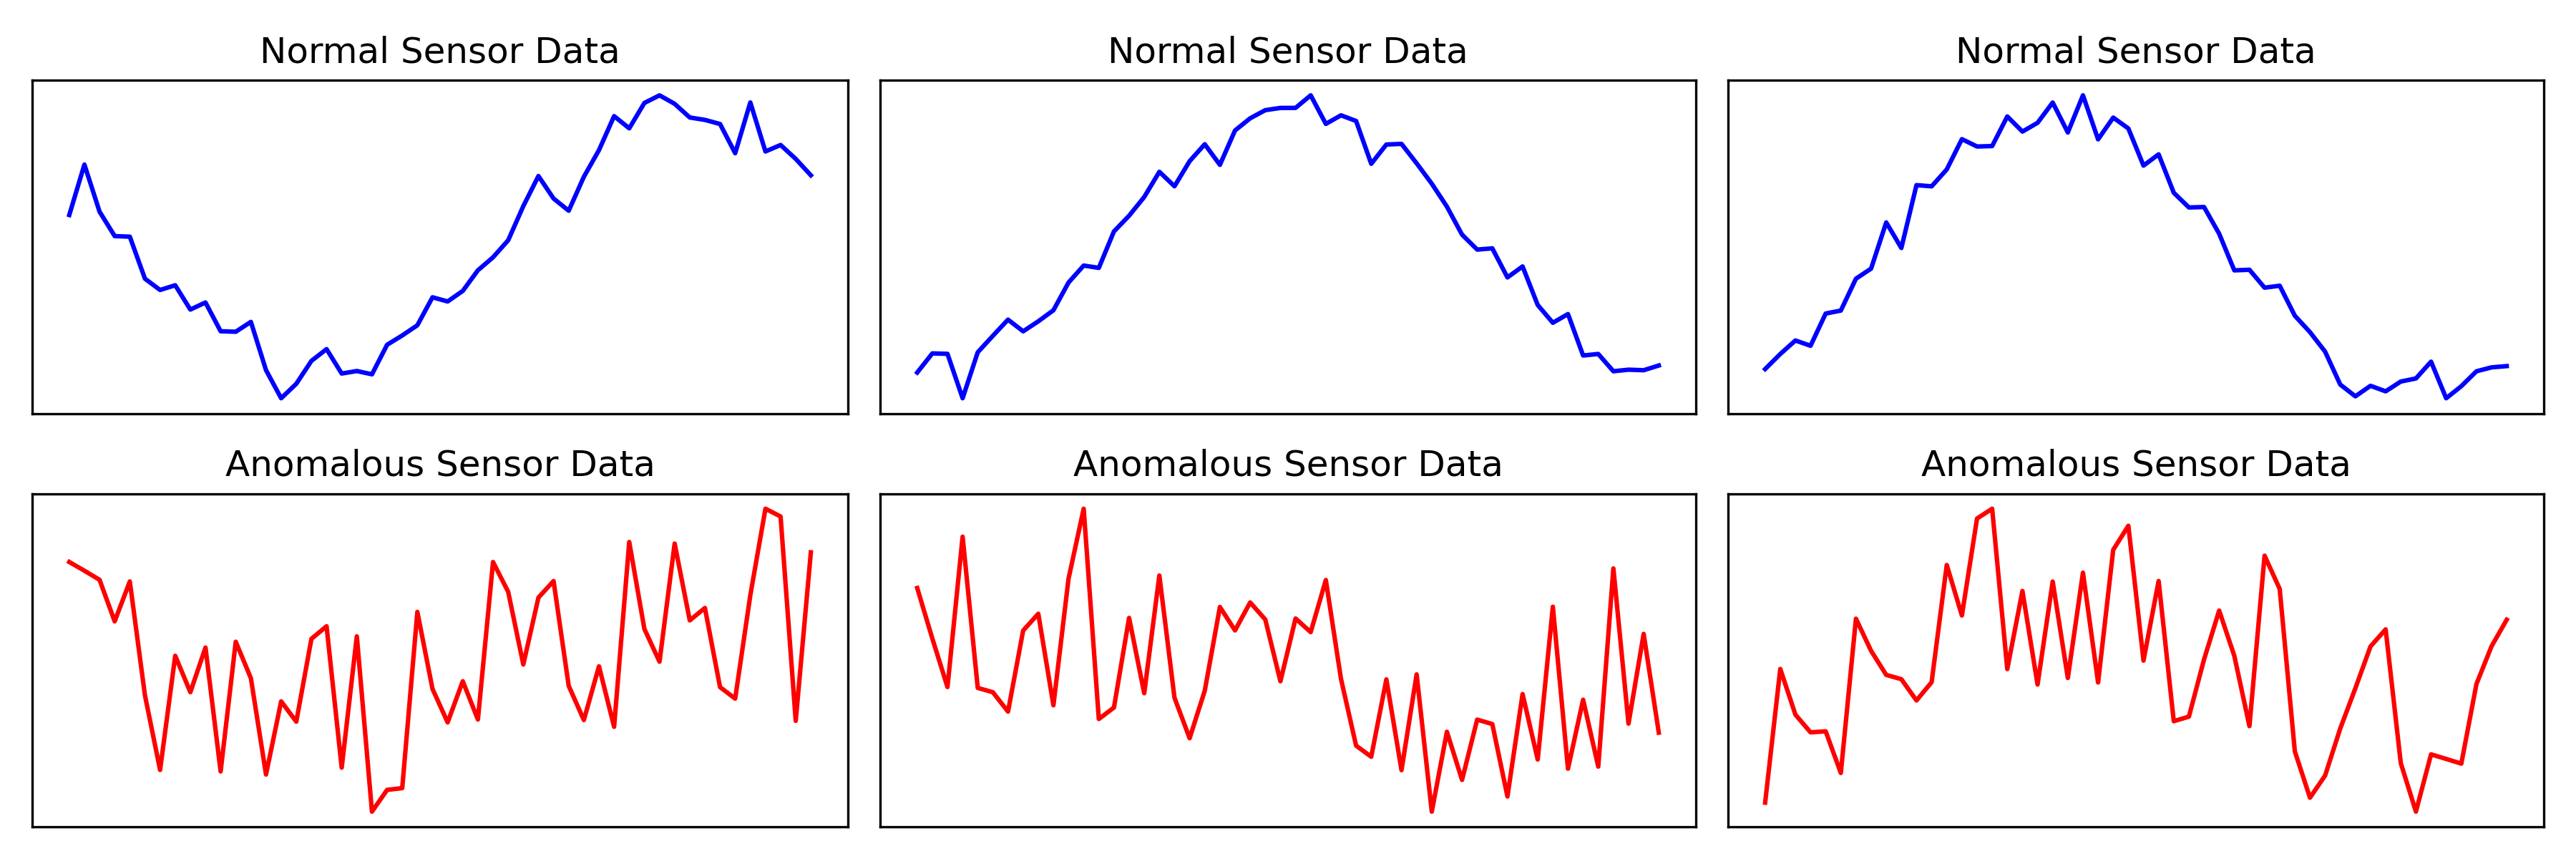
\includegraphics[width=0.9\textwidth]{images/lstm_sensor_data_samples.png}
    \caption{Examples of normal and anomalous sensor data. Normal sequences are in blue, while anomalies are shown in red.}
    \label{fig:sensor_data_samples}
\end{figure}

{\bf Defining the LSTM Autoencoder.} 
We define an LSTM autoencoder consisting of an encoder that compresses the input sequence into a lower-dimensional hidden state and a decoder that reconstructs the original sequence.

\begin{codeonly}{Defining the LSTM Autoencoder}
import torch

# Define device for computation (CPU/GPU)
device = torch.device("cuda" if torch.cuda.is_available() else "cpu")

class LSTMAutoencoder(nn.Module):
    def __init__(self, input_dim=1, hidden_dim=32, num_layers=2, seq_length=50):
        super(LSTMAutoencoder, self).__init__()
        self.seq_length = seq_length
        self.hidden_dim = hidden_dim
        self.num_layers = num_layers

        # LSTM layers
        self.encoder = nn.LSTM(input_dim,hidden_dim, num_layers,batch_first=True)
        self.decoder = nn.LSTM(input_dim,hidden_dim, num_layers,batch_first=True)

        # Final layer to reconstruct input
        self.output_layer = nn.Linear(hidden_dim, input_dim)

    def forward(self, x):
        batch_size = x.size(0)

        # Encode input
        _, (hidden, cell) = self.encoder(x)  # Correct hidden state extraction

        # Initialize decoder input as zeros
        decoder_input = torch.zeros(batch_size, self.seq_length, 1).to(x.device)

        # Decode using the last hidden state from the encoder
        decoder_output, _ = self.decoder(decoder_input, (hidden, cell))

        # Apply final layer to match original input size
        x_reconstructed = self.output_layer(decoder_output)

        return x_reconstructed  # Shape: [batch_size, seq_length, input_dim]

# Initialize model with correct sequence length
model = LSTMAutoencoder(seq_length=50).to(device)

\end{codeonly}

{\bf Training the Model.} 
The model is trained using Mean Squared Error (MSE) loss, optimizing the ability to reconstruct normal sequences.

\begin{codeonly}{Training the Model}
# Training setup
criterion = nn.MSELoss()
optimizer = optim.Adam(model.parameters(), lr=0.001)
num_epochs = 50
batch_size = 32

train_loader = torch.utils.data.DataLoader(X_train, batch_size=batch_size, shuffle=True)

# Track loss history
loss_history = []

# Training loop
for epoch in range(num_epochs):
    total_loss = 0
    for batch in train_loader:
        batch = batch.to(device)
        optimizer.zero_grad()
        outputs = model(batch)
        loss = criterion(outputs, batch)  # Compare input and output
        loss.backward()
        optimizer.step()
        total_loss += loss.item()

    epoch_loss = total_loss / len(train_loader)
    loss_history.append(epoch_loss)  # Store epoch loss
    print(f"Epoch {epoch+1}/{num_epochs}, Loss: {epoch_loss:.4f}")

plt.plot(loss_history, label="Loss")
plt.xlabel("Epochs"), plt.ylabel("Loss"), plt.title("LSTM Training Loss")
plt.legend(), plt.grid(True)
plt.savefig("lstm_training_loss.png", dpi=300)
plt.show()
\end{codeonly}

\begin{figure}[ht]
    \centering
    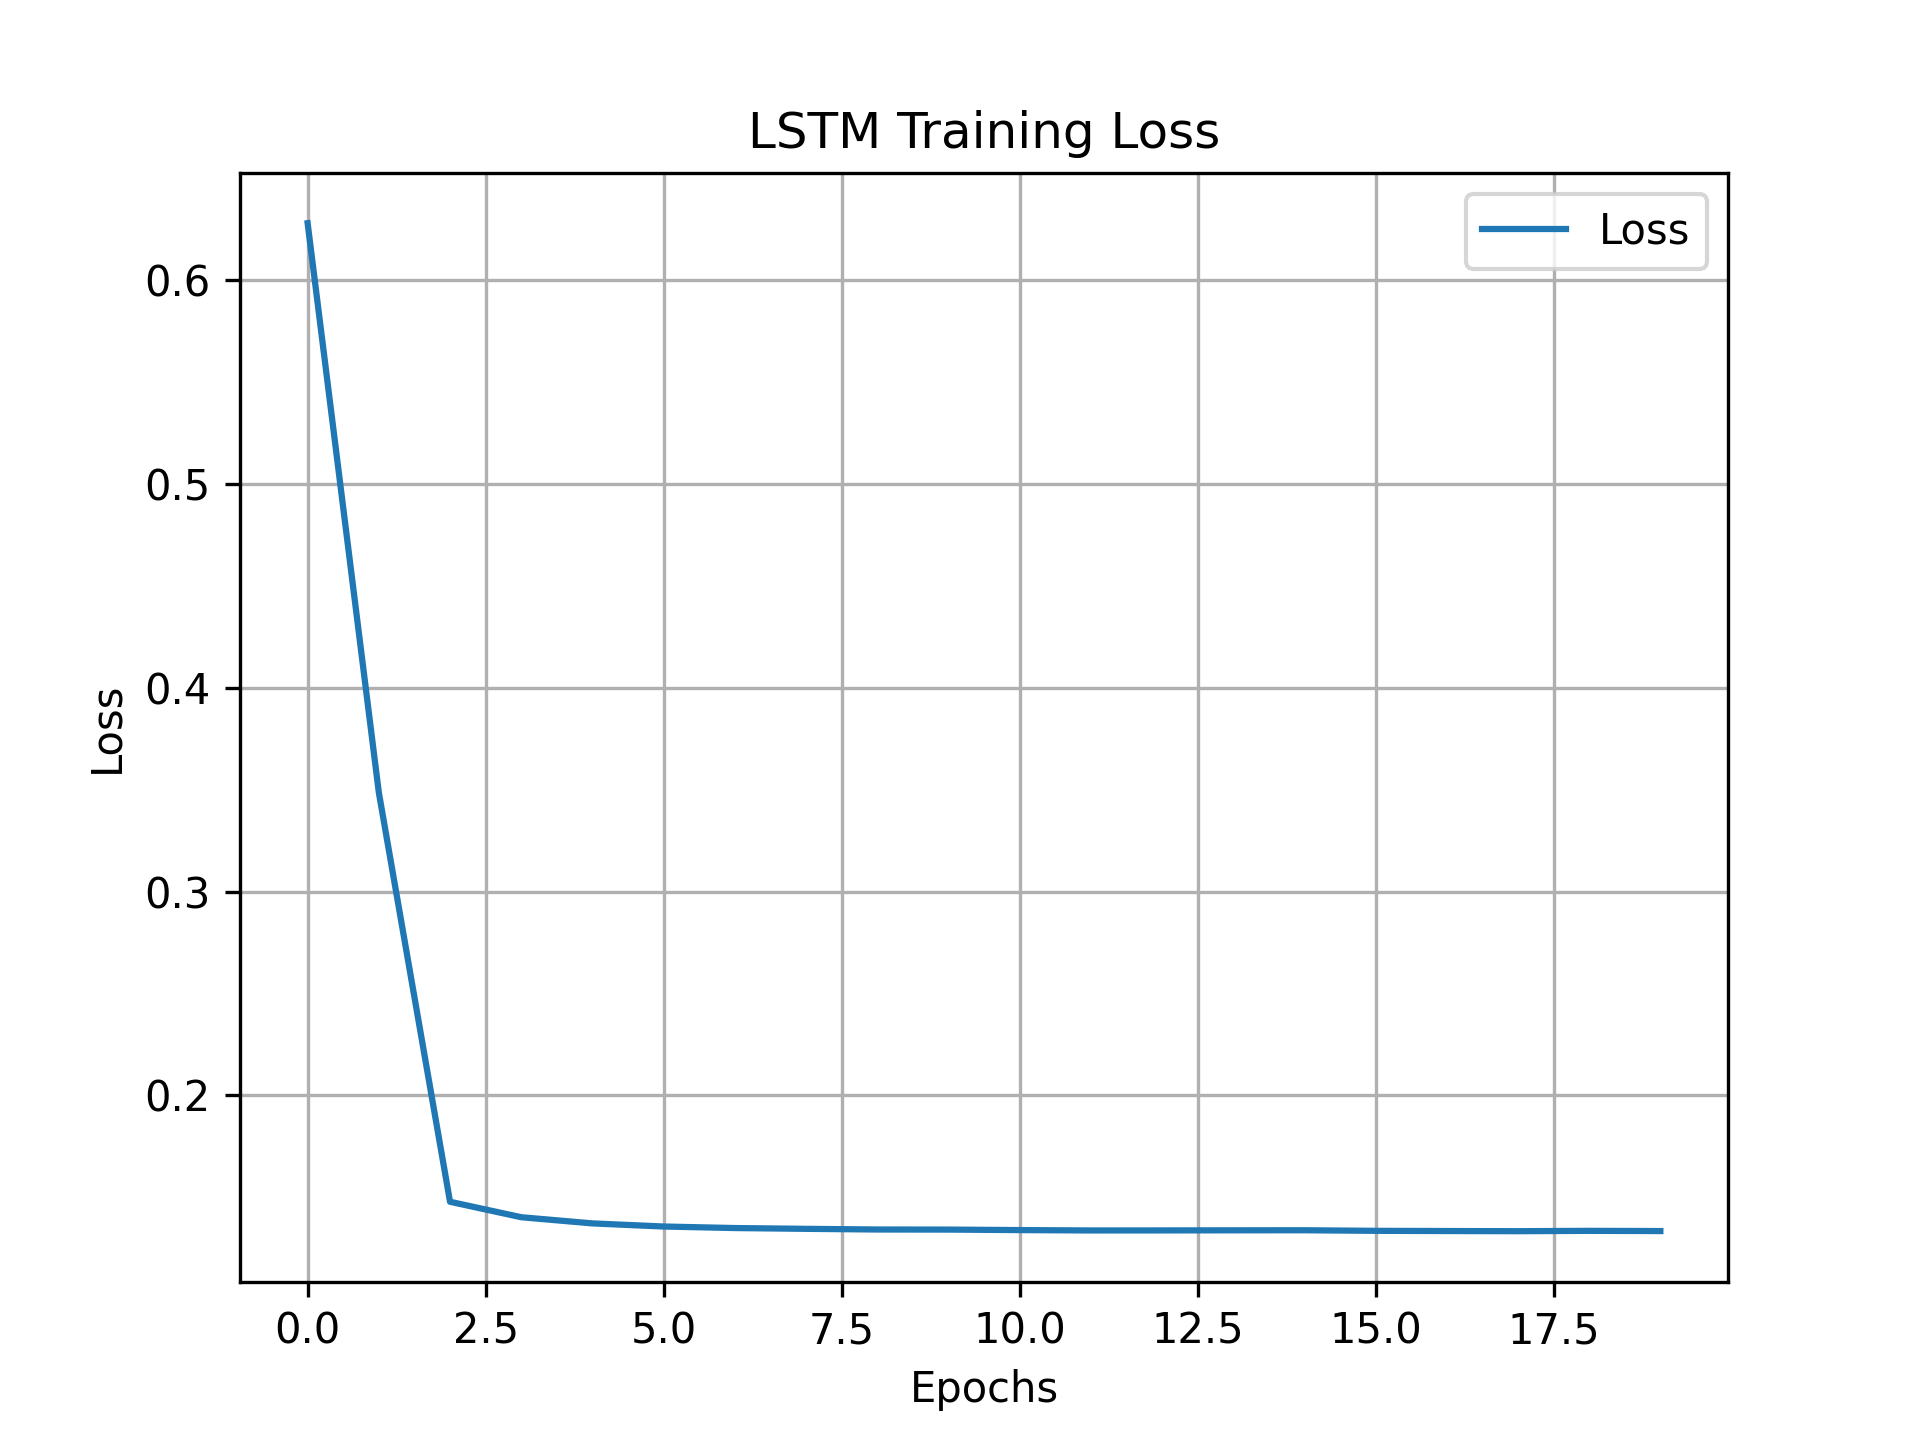
\includegraphics[width=0.9\textwidth]{images/lstm_training_loss.png}
    \caption{Training loss curve showing the decrease in reconstruction error over epochs.}
    \label{fig:training_loss}
\end{figure}

{\bf Detecting Anomalies.} 
Anomalies are detected by computing the reconstruction error on test sequences. If the error exceeds a predefined threshold (e.g., 95th percentile), the sequence is classified as an anomaly.

\begin{codeonly}{Anomaly Detection}
import numpy as np

# Compute reconstruction error on test data
model.eval()
X_test = X_test.to(device)
with torch.no_grad():
    X_reconstructed = model(X_test)

reconstruction_errors = torch.mean((X_test - X_reconstructed) ** 2, dim=(1, 2)).cpu().numpy()

# Set anomaly threshold (e.g., 95th percentile)
threshold = np.percentile(reconstruction_errors, 95)
y_pred = (reconstruction_errors > threshold).astype(int)  # 1 if anomaly, else 0

# Compute detection accuracy
accuracy = np.mean(y_pred == y_test) * 100
print(f"Anomaly Detection Accuracy: {accuracy:.2f}%")
\end{codeonly}

In our case we got 
\begin{verbatim}
Anomaly Detection Accuracy: 96.25%
\end{verbatim}

\begin{figure}[ht]
    \centering
    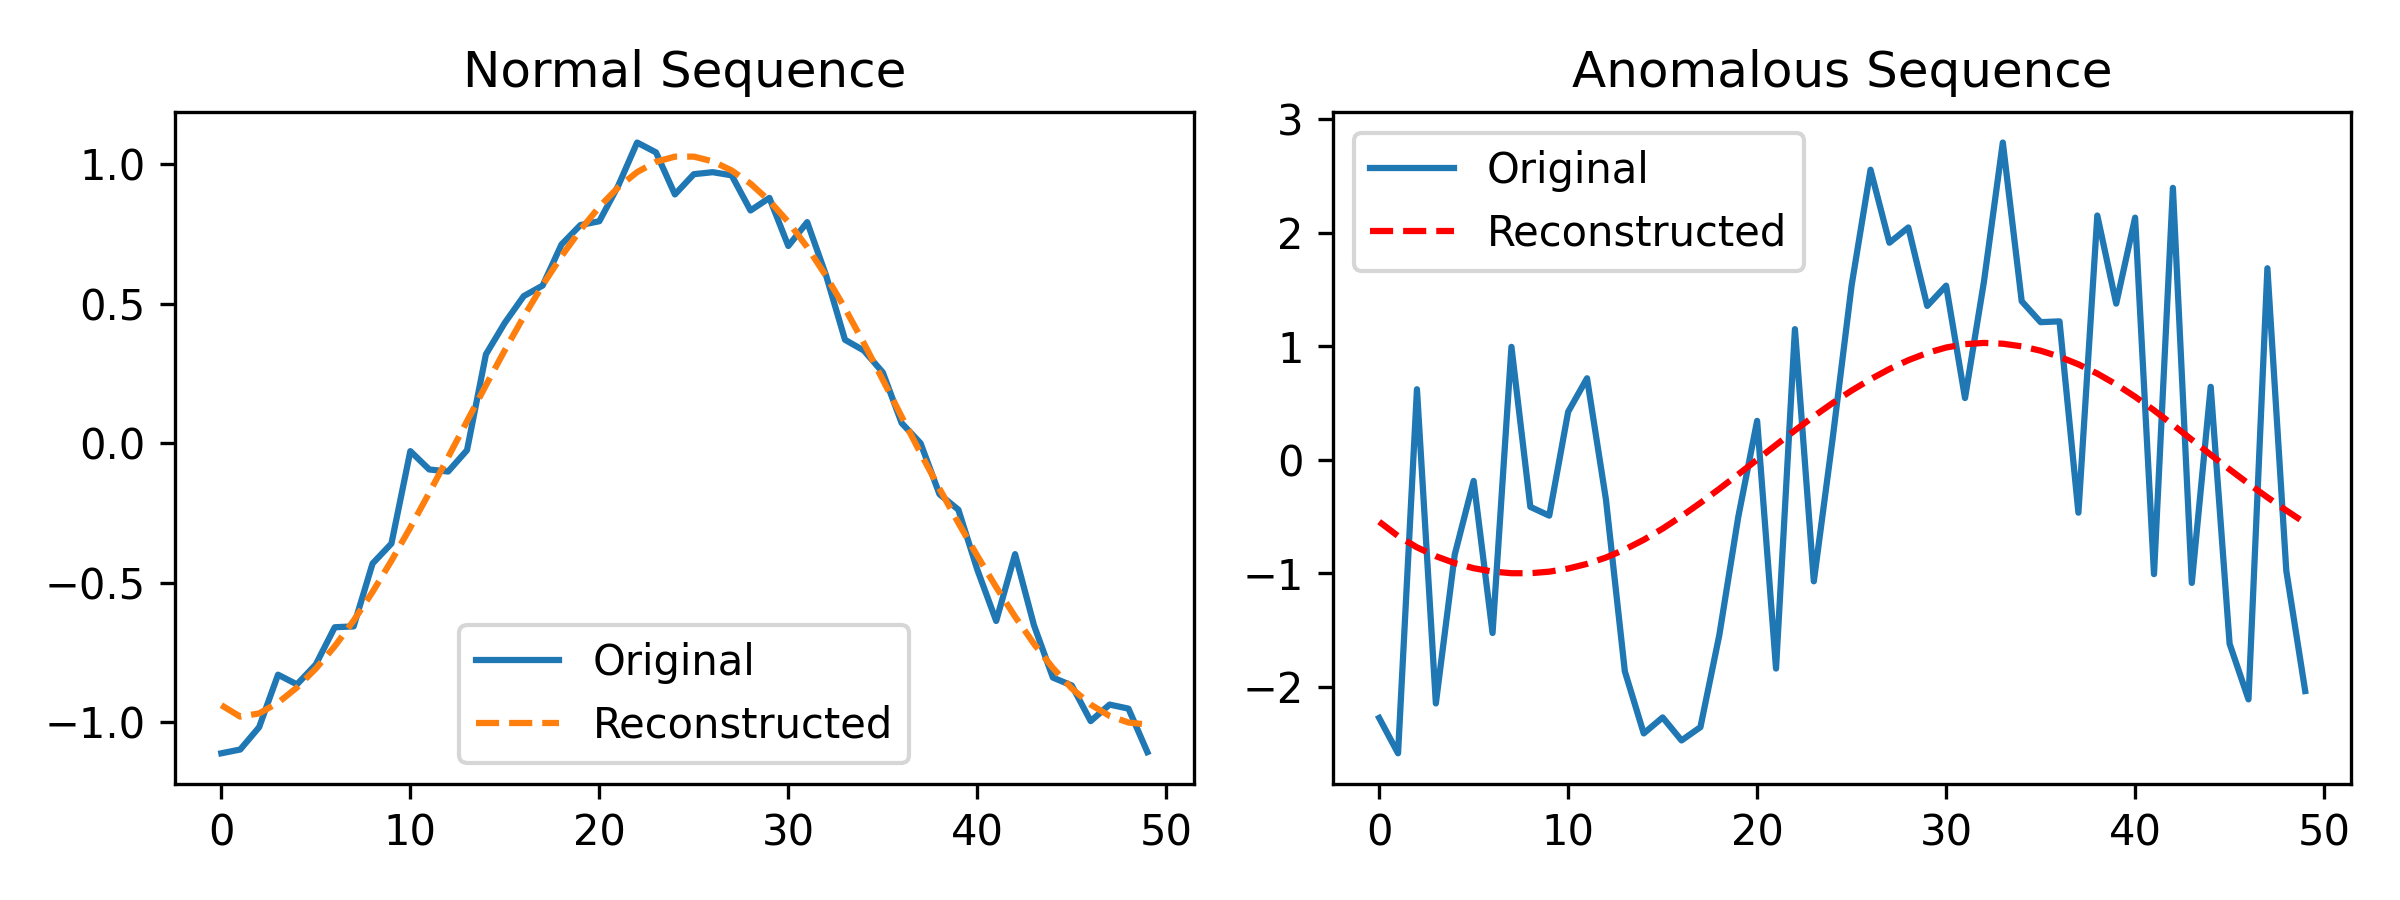
\includegraphics[width=0.9\textwidth]{images/lstm_anomaly_detection.png}
    \caption{Example of normal (left) and anomalous (right) sequences. Dashed lines represent reconstructed sequences.}
    \label{fig:anomaly_detection}
\end{figure}

{\bf Visualizing Detected Anomalies.} 
We randomly sample 12 sequences from the test set, classify them, and color them accordingly—blue for normal and red for anomalies.

\begin{figure}[ht!]
    \centering
    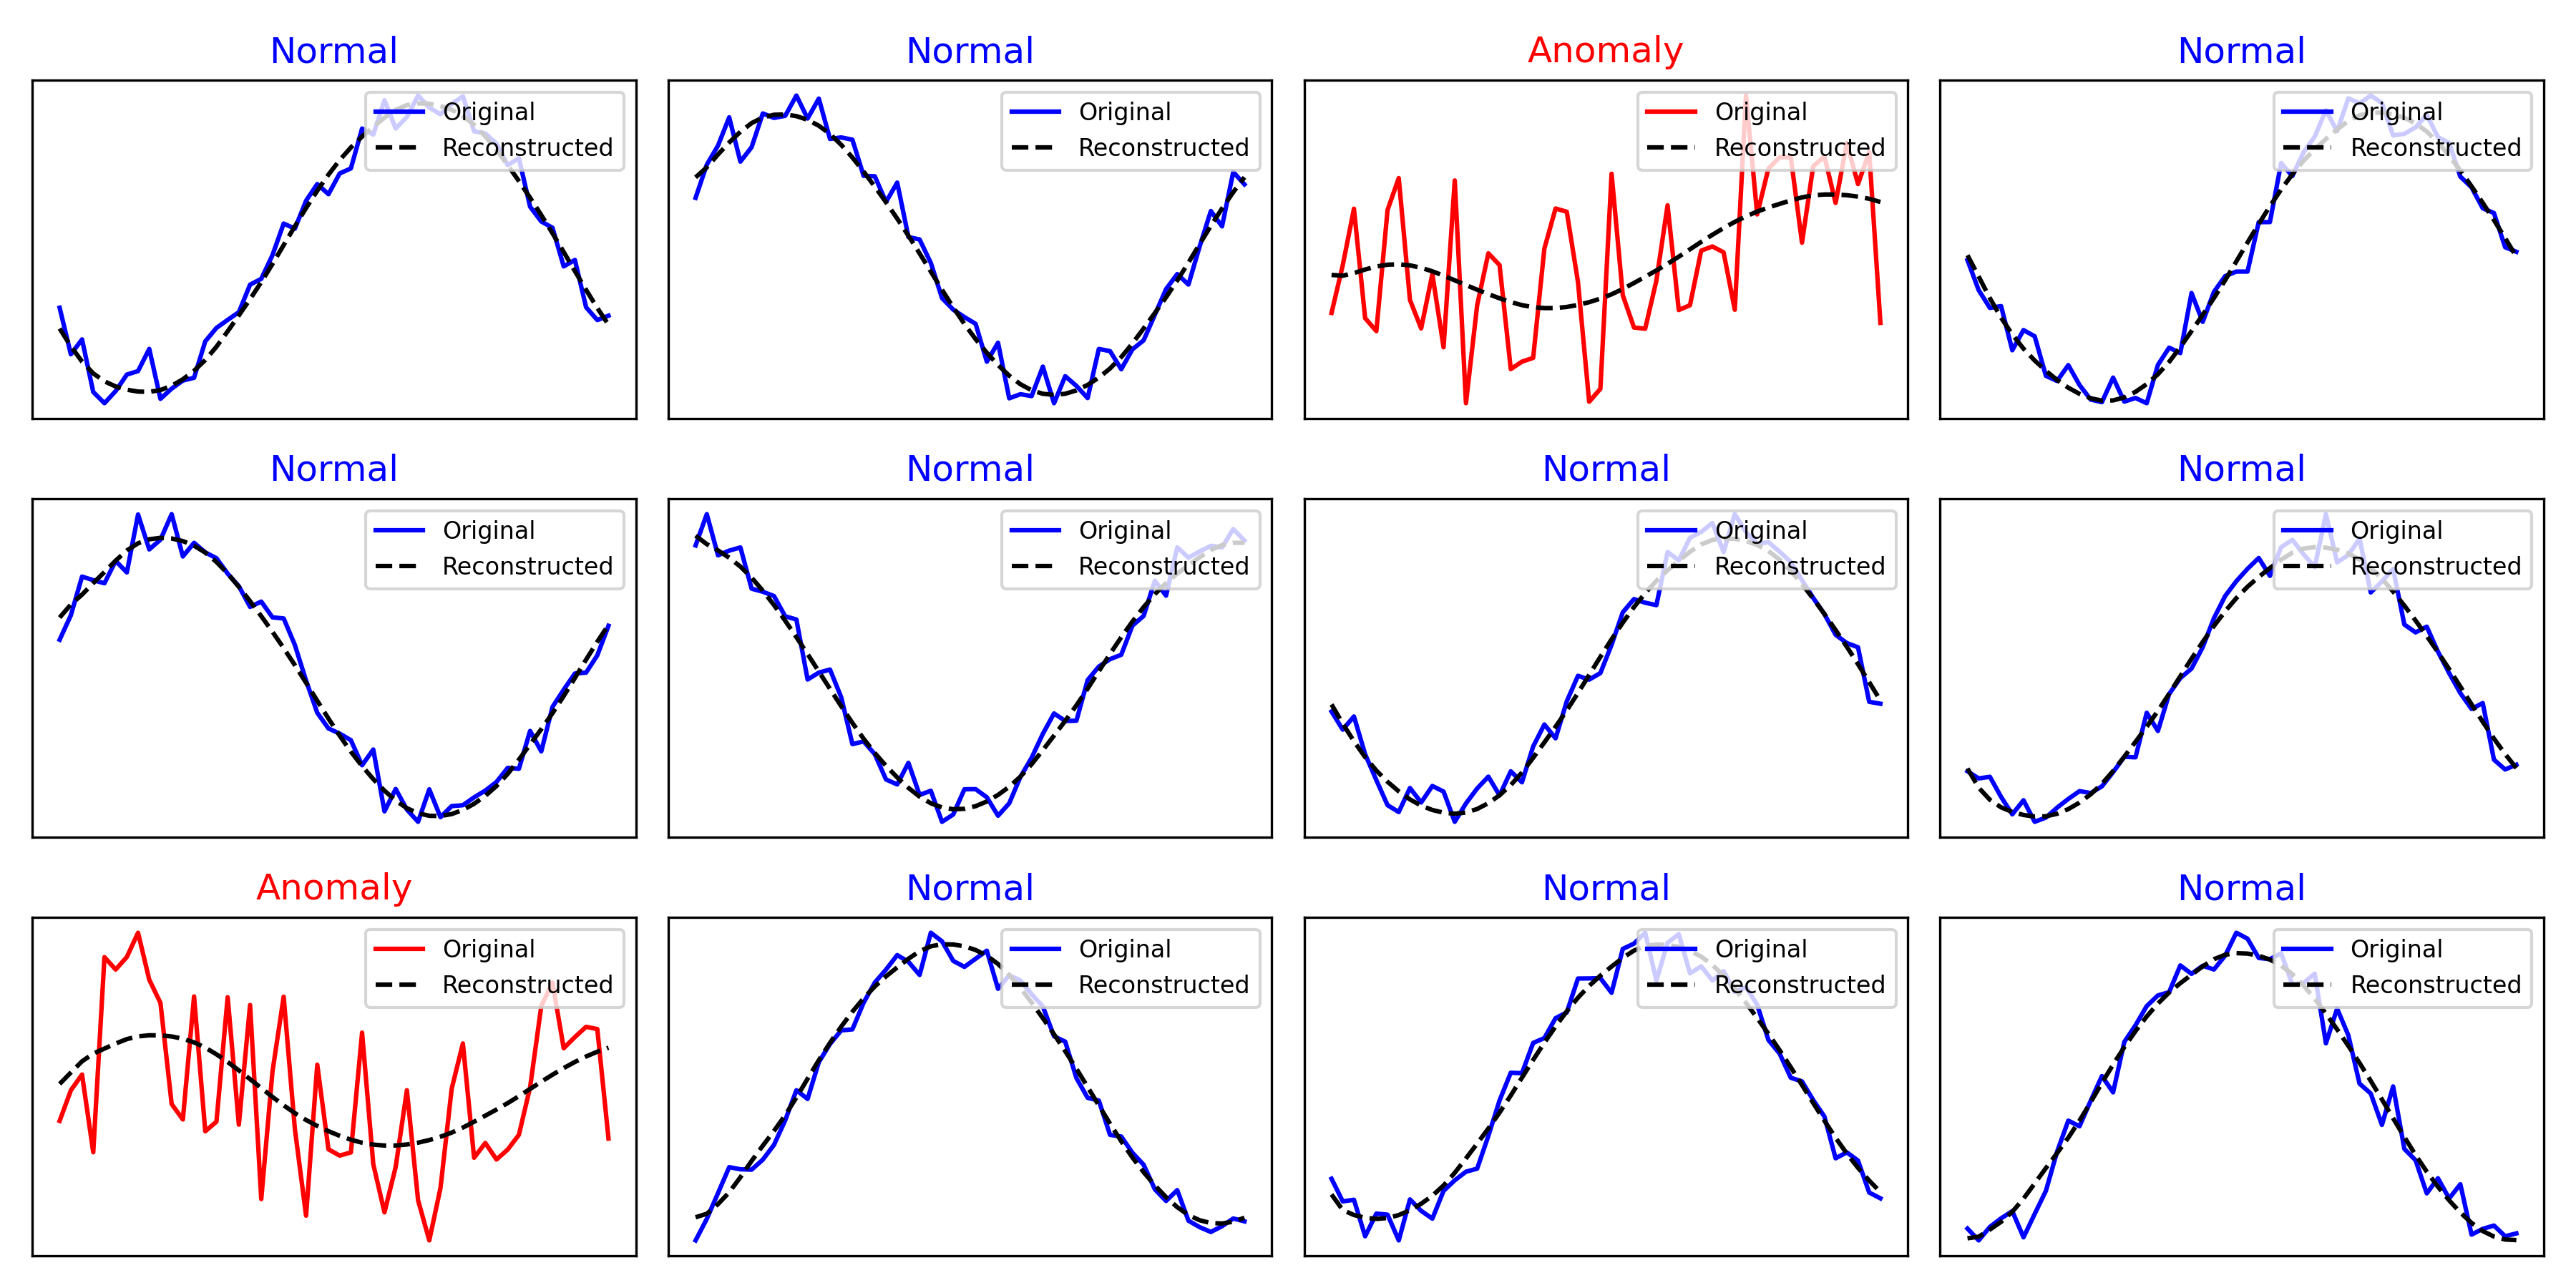
\includegraphics[width=0.9\textwidth]{images/lstm_anomaly_detection_samples_selected.png}
    \caption{Illustration of the detection and correction of the sensor anomaly.}
    \label{fig:training_loss}
\end{figure}


\begin{codeonly}{Visualizing Anomalies}
import matplotlib.pyplot as plt

# Select 12 random test samples
num_samples = 12
indices = np.random.choice(len(X_test), num_samples, replace=False)

# Compute reconstruction errors
model.eval()
with torch.no_grad():
    X_reconstructed = model(X_test.to(device))

reconstruction_errors = torch.mean((X_test - X_reconstructed) ** 2, dim=(1, 2)).cpu().numpy()

# Detect anomalies based on threshold
threshold = np.percentile(reconstruction_errors, 90)
y_pred = (reconstruction_errors > threshold).astype(int)  # 1 = Anomaly, 0 = Normal

# Plot the selected samples
plt.figure(figsize=(12, 6))
for i, idx in enumerate(indices):
    color = 'red' if y_pred[idx] == 1 else 'blue'
    
    plt.subplot(3, 4, i + 1)
    plt.plot(X_test[idx].cpu().numpy(), color=color, label="Original")
    plt.plot(X_reconstructed[idx].cpu().numpy(), linestyle="dashed", color="black", label="Reconstructed")
    plt.title(f"{'Anomaly' if y_pred[idx] == 1 else 'Normal'}", color=color)
    plt.xticks([]), plt.yticks([])
    plt.legend(fontsize=8, loc="upper right")

plt.tight_layout()
plt.savefig("lstm_anomaly_detection_samples_selected.png", dpi=300)
plt.show()
\end{codeonly}

\begin{recommendationbox}
There are quite different architectures of neural networks. The connectivity is a crucial choice for the functionality of the network. But also training datasets and optimisation strategies determine the success or failure of the network functionality and quality. 
\end{recommendationbox}

\begin{recommendationbox}
There is not one good or bad network or architecture, but different approaches are good for different applications. 
\end{recommendationbox}
